%%% File encoding: UTF-8
%% äöüÄÖÜß  <-- no German Umlauts here? Use an UTF-8 compatible editor!

%%% Magic comments for setting the correct parameters in compatible IDEs
% !TeX encoding = utf8
% !TeX program = pdflatex 
% !TeX spellcheck = en_US
% !BIB program = biber

\documentclass[master,english]{hgbthesis}
% Permissible options in [..]: 
%   Type of work: diploma, master (default), bachelor, internship 
%   Main language: german, english (default)
%%%----------------------------------------------------------

\RequirePackage[utf8]{inputenc}		% Remove when using lualatex or xelatex entfernen!
\usepackage{graphicx}
\usepackage{svg}
\usepackage{minted}
\usepackage{listings}
\usepackage{varioref}
\usepackage{longtable}
\usepackage{tabularx}

% -----------------------------------------------------
\newenvironment{code}{\captionsetup{type=listing}}{}
% -----------------------------------------------------
% -----------------------------------------------------
\newcommand{\mysubsubsection}[1]{{\subsubsection{\textbf{#1}}}}
\newcommand{\mentionedtext}[1]{{\textit{{#1}}}}
\newcommand{\sourceDir}{./sources}
\newcommand{\sourceFontSize}{\fontsize{10pt}{11.5}}
\newmintedfile[bashFile]{bash}{
	linenos=false, 
	frame=none, 
	breaklines=true, 
	tabsize=2,
	numbersep=5pt,
	xleftmargin=10pt,
	baselinestretch=1,
	fontsize=\sourceFontSize
}
\newmintedfile[yamlFile]{yaml}{
	linenos=false, 
	frame=none, 
	breaklines=true, 
	tabsize=2,
	numbersep=5pt,
	xleftmargin=10pt,
	baselinestretch=1,
	fontsize=\sourceFontSize
}
\newmintedfile[javaFile]{java}{
	linenos=false, 
	frame=none, 
	breaklines=true, 
	tabsize=2,
	numbersep=5pt,
	xleftmargin=10pt,
	baselinestretch=1,
	fontsize=\sourceFontSize
}
\newmintedfile[xmlFile]{xml}{
	breaklines=true, 
	tabsize=2,
	numbersep=5pt,
	xleftmargin=10pt,
	baselinestretch=1,
	autogobble=true,
	breakautoindent=false,
	fontsize=\sourceFontSize
}
\newmintinline[inlineJava]{java}{
	fontsize=\sourceFontSize
}
\newmintinline[inlineBash]{bash}{
	fontsize=\sourceFontSize
}
% -----------------------------------------------------
\graphicspath{{images/}}    % location of images and graphics
\logofile{logo}				% logo file = images/logo.pdf (use \logofile{} for no logo)
\bibliography{references.bib}  	% name of bibliography file (references.bib)
\setlength{\parindent}{0pt}

%%%----------------------------------------------------------
% Title page entries
%%%----------------------------------------------------------

%%% Entries for ALL types of work: --------------------------
\title{Implementation of an Enterprise Service Bus with OpenShift} %no camel used (and Camel)
\author{Ing. Thomas Herzog B.Sc}
\programname{Software Engineering}
\placeofstudy{Hagenberg}
\dateofsubmission{2018}{06}{01}	% {YYYY}{MM}{DD}

%%% Entries for Bachelor theses only: -----------------------
%\thesisnumber{XXXXXXXXXX-A}   %e.g. 1310238045-A  
% (Stud-ID, A = 1st Bachelor thesis)
%\semester{Fall Semester 2017} 	% Fall/Spring Semester YYYY
%\coursetitle{Introduction to Trivial Problems 1} 
\advisor{DI (FH) Peter Kulczycki}

%%% Restricted publication license instead of CC (master only):
\strictlicense

%%%----------------------------------------------------------
\begin{document}
%%%----------------------------------------------------------

%%%----------------------------------------------------------
\frontmatter							% title part (roman page numbers)
%%%----------------------------------------------------------

\maketitle
\tableofcontents

%\chapter{Preface}






 	% preface is optional
\chapter{Abstract}
An Enterprise Service Bus (ESB) is a crucial part of an enterprise, which connects the enterprise to its partners, customers, and other branches. The appearance of containerization, cloud services, and the microservice architecture have provided new possibilities for implementing and running an ESB. But, an ESB is commonly used by large conservative enterprises, which don't adapt new technologies fast, and wait until a new technology has proven itself. Especially the cloud is something the industry denied to use for a long time, because of the fact, that the infrastructure and data are managed and maintained by external service providers. \\ 

These days, we live in the so called cloud age, whereby global enterprises like Red Hat or Amazon provide cloud services such as Platform as a Service (PaaS), which can scale with the business. Enterprises start to consider to move their ESB installations to the cloud to profit from the cloud service provided features. Moving an ESB to the cloud will be a long term process for an enterprise, because the established processes for development, running, and managing the ESB will have to change. \\

This thesis has the goal to give the reader an overview of the cloud related concepts and technologies such as, Infrastructure as Code (IaC) and Docker, which are the base for cloud services. The implemented ESB prototype,  is  available at \url{https://github.com/cchet-thesis-msc/prototype}, and shows how an ESB could be implemented on a PaaS platform. \\




%%%----------------------------------------------------------
\mainmatter          			% main part (arabic page numbers)
%%%----------------------------------------------------------

\chapter{Introduction}
\label{cha:intro}

\section{Motivation}
\label{sec:intro-motivation}
Large enterprises work with several independent applications, whereby each application covers an aspect of their business. In general, these applications are from different vendors, implemented in different programming languages, and with their own life-cycle management. To provide a business value to the enterprise, these applications are connected via a network, and they contribute to a business workflow. The applications have to exchange data, which is commonly represented in different formats and versions. This leads to a highly heterogeneous network of applications, which is hard to maintain. \\

The major challenge of an IT department is the integration of independent applications into the enterprise application environment. The concept of Enterprise Application Integration (EAI) provides patterns, which help to define a process for the integration of applications into a heterogeneous enterprise application environment. One of these patterns is the Enterprise Service Bus (ESB), which is widely used in the industry\cite{EIP}. \\

Often, the term ESB application is used to refer to an ESB, which integrates internal and external hosted applications. But an ESB is a software architectural model, rather than an application. The term could have been established by the usage of middleware such as JBoss Fuse, which provides tooling to integrate applications into an ESB. Red Hat JBoss Fuse is be based on the JBoss Enterprise-Application-Platform (JBoss EAP), where all integration services run in the same runtime environment\cite{Fuse2018}. \\

With the appearance of cloud solutions, such as Platform as a Service (PaaS), it is now possible to move an ESB from a dedicated environment to a cloud environment, whereby each integration service runs in its own runtime environment, rather than joining an existing runtime environment. The concept of Integration Platform as a Service (IPaaS) is built on top of PaaS, and enhances a common PaaS solution with the integration features required by EAI\cite{PaaS2015, iPaaSP12015}. \\

Thus, enterprises can reduce the effort in implementing and maintaining an ESB, integrating applications into the ESB, and reducing the costs of an ESB, by using a consumption based pricing model. The cost are reduced due to the fact, that the ESB can scale down when its load decreases, whereby less resources are consumed, which have to be paid for.

\section{Objectives}
\label{sec:intro-objectives}
This thesis aims to implement an ESB on Openshift PaaS. An ESB is different to a Service Hub, because the ESB is a distributed system by design, whereby for instance, transformation is not centralized, as it is with an Service Hub. A Service Hub has a central component, which performs transformation, routing and orchestration, whereby the scaling is limited by the hardware capabilities of the central hub. Additionally, the hub component of a Service Hub represents a single point of failure\cite{EIP}. \\

Commonly, an ESB is implemented with the help of middleware such as JBoss Fuse, which is based on the JBoss EAP. The concepts of PaaS and IPaaS are in general new to the industry, which commonly hosts their integration services in their own data centers, due to the lack of trust for cloud solutions and knowledge about the new approaches such as the microservice architecture\cite{Openshift2018}. \\

Before implementing an ESB, which runs on a PaaS platform such as Openshift, it is necessary to understand the new concepts such as Infrastructure as Code (IaC) or containerization with Docker, which are covered in the following chapters. The microservice architecture and cloud services such as PaaS are becoming more important for the software industry, because of the features they provide. For instance, Red Hat is currently moving its ESB middleware JBoss Fuse to the cloud, whereby JBoss Fuse will fully rely on Openshift, and the integration services will have to be implemented as microservices. This has a huge impact on Red Hats customers, who are used to JBoss Fuse on top of JBoss EAP. \\

This thesis was commissioned by the company Gepardec IT Services GmbH, a company, which is working in the area of Java Enterprise and Cloud Development. The migration from a monolithic ESB to a microservice structured ESB, which is hosted in a PaaS environment, is a major concern for them. The migration from a monolithic ESB to a microservice structured ESB will be a major challenge for their customers, because microservice architecture and cloud solutions are mostly new to them.  \\

Over the past years a huge technology dept has been produced by the industry, due to the monolithic architecture of their applications and little refactoring work on their application sources. It will be hard for them to reduce the accumulated technology dept, which they will have to, to keep competitive. Gepardec sees a lot of potential for their business and their customers in this new approach of implementing and hosting an ESB. \\

The term \quotes{monolithic ESB} refers to an ESB implementation, whereby all integration services are part of a single application, and therefore, are part of the application life-cycle, instead of having an own life-cycle per integration service. An integration service is a service, which integrates two or more other service with each other, by handling aspects like data transformation, routing, or security, between the integrated services.  
\chapter{Infrastructure as Code}
\label{cha:iac}
Infrastructure as Code (IaC) is a concept to automate system creation and change management with techniques from software development. Systems are defined in a Domain Specific Language (DSL), which gets interpreted by a tool, which creates an instance of the system or applies changes to it. IaC defines predefined, repeatable routines for managing systems \cite{Morris2016}. IaC descriptions are called templates, cookbooks, recipes or playbooks, depending on the tool. In the further course, the IaC definitions will be called templates. The DSL allows to define resources of a system such as network, storage and routing descriptively in a template. The DSL abstracts the developer from system specific settings and provides a way to define the system with as little configuration as possible. The term system is used as a general description. In the context of IaC, a system can be anything which can be described via a DSL.

\section{The Need for Infrastructure as Code}
\label{sec:iac-need}
In the so called iron age, the IT systems were bound the physical hardware and the setup of such a system and its change management were a long term, complex and error prone process. These days, we call such systems legacy systems. In the cloud age, the IT systems are decoupled from the physical hardware and in the case of PaaS they are even decoupled from the operating system \cite{Morris2016}. The IT systems are decoupled from the physical hardware and operating system, due to the fact, that cloud providers cannot allow their customer to tamper with the underlying system and hardware. In general, the hardware resources provided by a cloud provider are shared by multiple customers. \\

With IaC it is possible to work with so called Dynamic Infrastructure Platforms, which provide computing resources, where the developers are completely abstracted from the underlying system. Dynamic infrastructure platforms have the characteristic to be programmable, are available on-demand and provide self service mechanisms, therefore we need IaC to work with such infrastructures \cite{Morris2016}. Systems deployed on a dynamic infrastructure platform are flexible, consistent, automated and reproducible. \\

Enterprises which stuck to legacy systems face the problem that technology nimble competitors can work with their infrastructures more efficiently, and therefore can demand lower prices from their customers. This is due to the IaC principles discussed in Section \vref{sec:iac-principles}. Over a short period of time, enterprises will have to move to IaC and away from their legacy systems to stay competitive. The transition process could be challenging for an enterprise, because they lose control over the physical hardware and maybe also over the operating system. Maintaining legacy systems has the effect that someone is close to the system and almost everything is done manually. IaC has the goal to automate almost everything, which requires trust for the cloud providers, who provide the computing resources and the tooling, which provides the automation. A well known problem, which enterprise will face, is the so called Automation Fear Spiral, which is shown in Figure \vref{fig:automation-fear-spiral}.

\begin{figure}[htbp]
	\centering
	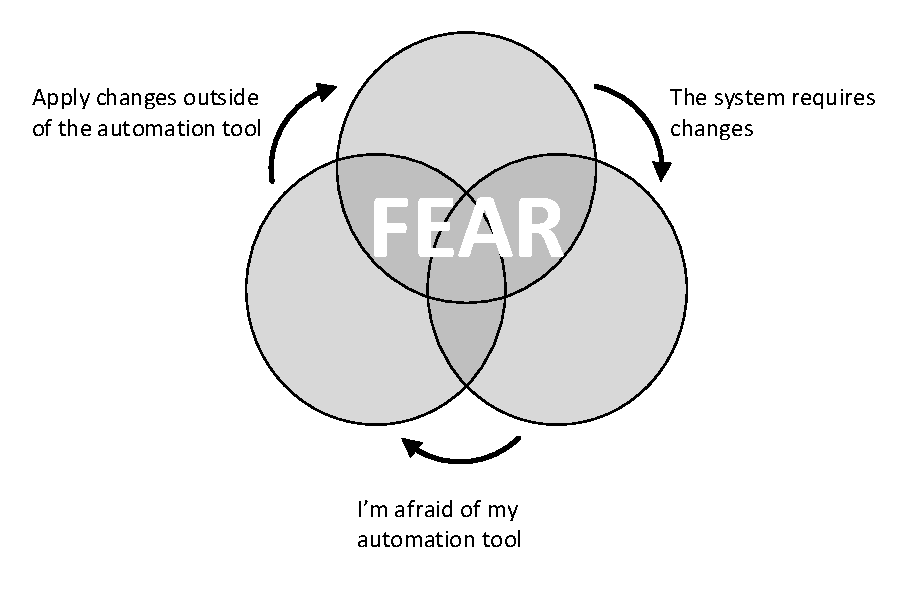
\includegraphics[scale=1]{images/automation-fear-spiral.pdf}
	\caption{Automation Fear Spiral}
	\label{fig:automation-fear-spiral}
\end{figure} 

Because of no trust for the automation, changes are applied manually to the systems and outside the defined automation process. If the system is reproduced, definitions may be missing in the templates, which leads to an inconsistent system. Therefore, enterprises have to break this spiral to fully profit from IaC \cite{Morris2016}. \\

When enterprises have moved their legacy systems to IaC, they can not only manage their systems faster, they also can profit from the principles of IaC as discussed in Section \vref{sec:iac-principles}. With IaC, systems are less complicated to manage, changes can be applied without fear, and the systems can easily be moved between environments. This provides the enterprises with more space to maneuver, systems can become more complex but still easy to manage, the systems can be defined and created faster which could lower costs.    

\section{Principles of Infrastructure as Code}
\label{sec:iac-principles}
The principles of IaC solve the problems of systems of the iron age. In the iron age the creation and maintenance of systems were a long, complicated and error prone process which consumed a lot of resources and time. With the decoupling of the physical hardware from the system, the creation and maintenance of the system has become simple, due to the IaC DSL and tooling. 

\subsection{Infrastructures are Reproducible}
\label{sec:iac-principles-reproducibility}
With IaC, systems are easy reproducible. It is possible to reproduce the whole infrastructure or parts of it effortlessly. Effortless means, that no tweaks have to be made to the templates or during the reproduction process and there is no need for a long term decision process about what has to be reproduced and how to reproduce it. To be able to reproduce system effortlessly is powerful, because it can be done automatically, consistently and with less risk of failures \cite{Morris2016}. The reproducibility of a system is based on reusable templates which provide the possibility to define parameters, which are set for the different environments as shown in Figure \ref{fig:reproduce-infrastructure}.

\begin{figure}[htbp]
	\centering
	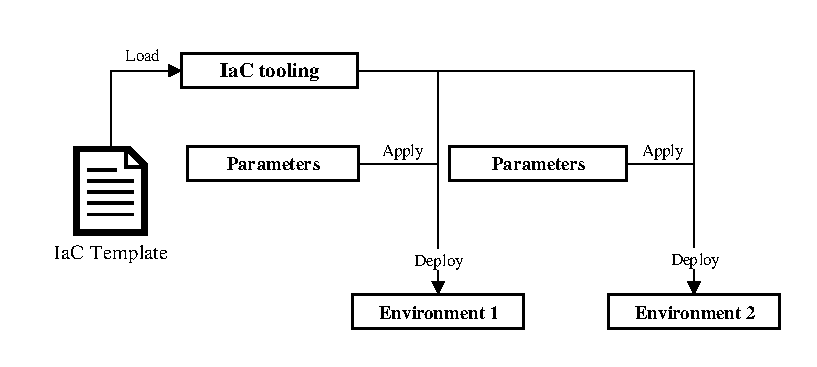
\includegraphics[scale=0.95]{images/reproduce-infrastructure.pdf}
	\caption{Schema of a parametrized infrastructure deployment}
	\label{fig:reproduce-infrastructure}
\end{figure} 

\subsection{Infrastructures are Disposable}
\label{sec:iac-principles-disposable}
Another benefit of IaC is that systems are disposable. Disposable means, that systems can be easily destroyed and recreated. Changes made to the templates of a system does not have to be applied on an existing system, but can be applied by destroying and recreating the system. An requirement for a disposable system is, that it is understood that systems will always change. Other systems relying on a disposable system need to address that the system could change at any time. Systems must not fail because a disposable system disappears and reappears again because of an redeployment \cite{Morris2016}.

\subsection{Infrastructures are Consistent}
\label{sec:iac-principles-consistency}
Systems managed with IaC are consistent, because they are defined via a template and all instances are an instance of the template, with the little configuration differences defined by parameters. As long as the system changes are managed by IaC, the system will stay consistent, and the automation process can be trusted. \\

In Listing \vref{src:iac-template-docker-compose} an example for an IaC template is shown, which defines a Docker Compose service infrastructure for hosting a Wildfly server instance \cite{Wildfly2017, DockerCompose2018}. This system can consistently be reproduced on any environment supporting Docker, Docker Compose and providing values for the defined parameters. \\

\begin{code}
	\yamlFile{\sourceDir/iac-docker-compose.yml}
	\caption{Example for an IaC template for Docker Compose}
	\label{src:iac-template-docker-compose}
\end{code}

\subsection{Actions are Repeatable}
\label{sec:iac-principles-repeatability}
Building reproducible systems, means that any action applied to the system should be repeatable. Without repeatability, the automation cannot be trusted and systems wouldn't be reproducible. An instance of a system in another environment should be equal to any other system instance, except for the configurations defined by parameters. If this is not the case, then a system is not reproducible, because it will have become inconsistent \cite{Morris2016}. \\

IaC is a concept which makes it very easy to deal with systems in the cloud age. Enterprises can make use of IaC to move their legacy systems to the cloud, where they can profit from the principles of IaC. Nevertheless, before an enterprise can profit from IaC, it has to apply clear structures to their development process, as well as sticking to the principles of consistency and repeatability. For experienced administrators, who are used to maintain systems manually, it could sometimes be hard to understand why they are not supposed to perform any actions on the system manually anymore, nevertheless that a manual change could be performed faster. Being capable to reproduce a system at any time with no effort,  or applying changes on an existing system in a predefined and consistent manner,  makes enterprises very flexible and fast. Enterprises will not have to fear future changes in requirements and technologies of their systems anymore.    




\chapter{Containerization with Docker}
\label{cha:containerization-docker}
Docker is a tool for creating, provisioning and interacting with Linux Containers (LXC) \cite{Docker2018,LXC2018}. LXC are a lightweight version of virtualization, which does not have the resource impact of a full virtualization such as Operating System (OS) virtualization. The differences of LXC and a Virtual Machine (VM) are covered in Section \ref{sec:docker-virtualization-vs-containerization}. Docker has become very popular over the past years, due to the fact, that it made it possible to easily work with LXC. Docker relies strongly on the principles of IaC which has been discussed in Chapter \ref{cha:iac}. When using Docker, Linux Containers are often referred to as Docker Containers. \\

Containerization is a key factor when hosting applications in the cloud, because the applications are normally packaged in images and run as containers on the cloud platform. Containerization provides features for a fast, effortless and consistent way of running applications in the cloud, which is discussed in the following Section \ref{sec:docker-need-for-containerization}.

\section{The need for Containerization}
\label{sec:docker-need-for-containerization}
Containerization is a key factor for cloud platforms such as PaaS, where each application runs in its own isolated environment, called a container. A container is an instance of an image, which represents the initial state of an application. A VM represents a full blown OS, where the OS provides a kernel, which is emulated on the host OS by the Hypervisor. A Hypervisor is a software which can create, run and manage VMs. A container uses the kernel provided by the host OS and therefore there is no need for an emulation. A container does not represent a full blown OS, but still provides features normally provided by an OS such a networking and storage \cite{DockerVirtScheepers2014}. \\ 

Containers are faster to create, to deploy and easier to manage compared to VMs. Nevertheless, cloud platforms use virtualization for managing their infrastructure, where the containers run on the provisioned VMs. The usage of containers compared to the usage of VMs can reduce costs for hosting applications. Enterprises can profit from hosting their applications of containers in several ways. Applications hosted in containers need lees resources than applications hosted in VMs, because there is no virtualized OS and no need for kernel emulation. The creation, deployment and startup of containers are faster, because only the isolated process needs to be started and not a full blown OS. Docker is well supported by Integrated Development Environments (IDEs), which provide support for creating Docker Image definitions (Dockerfiles) and provisioning of Docker Containers on a local or remote environment \cite{DockerFile2018}. \\

When enterprises have applied IaC to their infrastructure, then the next logical step is to integrate their applications into IaC as well. Applications hosted in containers profit from the IaC principles immutability, reproducibility, repeatability and consistency. Therefore, Docker strongly relies on IaC and provides tooling for automating creation and provisioning of Docker Containers, which is used by PaaS platforms such as Openshift. With Docker, developers define the hosting environment for their applications and not system administrators anymore. Nevertheless, developers can profit from the deep Linux knowledge of system administrators, to define the Docker Images efficiently, to keep them small and secure. The following Section \ref{sec:docker} will give an overview of the Docker technology, its architecture and artifacts.  

\section{Docker}
\label{sec:docker}
This section covers Docker, which is the most popular tool to work with LXC. Docker is open source but also provides an enterprise support. The core part of the Docker technology is the Docker Engine, which is discussed in Section \ref{sec:docker-engine}. The Docker Engine is the part of the Docker technology that actually runs the containers. The Docker Images are managed in a so called Docker Registry, which is a repository for Docker Images. The most popular Docker Registry is Docker Hub, which is a free service, where anyone can provides Docker Images \cite{DockerRegistry2018}.

\subsection{Docker Engine}
\label{sec:docker-engine}
Figure \ref{fig:docker-engine} illustrates the Docker Engine architecture hosted on a Linux OS. The Docker Engine is build by layers, where each layer communicates with the layer beneath.

\begin{figure}[htbp]
	\centering
	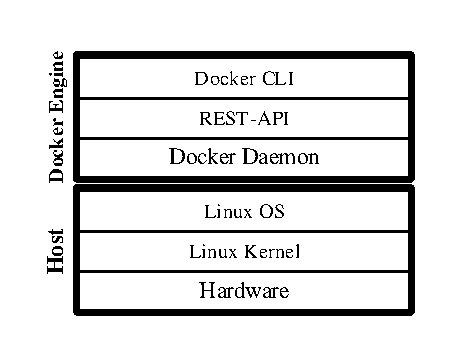
\includegraphics[scale=0.8]{images/docker-engine.pdf}
	\caption{Docker Engine architecture}
	\label{fig:docker-engine}
\end{figure} 

The Docker Engine was initially designed for LXC exclusively but has been ported to Windows. Docker Images and Containers created for Windows OS are not supported on a Linux OS and visa versa. The Docker Images and Containers for a Windows OS differ from those for a Linux OS, but the principles of Docker Images and Docker Containers are the same.

\mysubsubsection{Docker Daemon}
\label{sec:docker-daemon}
The Docker Daemon represents the background process, which creates, runs and manages the Docker Containers on the Docker Host, similar to a VM Hypervisor. The Docker Daemon strongly depends on the kernel of the host OS, therefore incompatibilities could cause the Docker Daemon to fail functioning. The communication with the Docker Daemon is performed via a REST-API, because the Docker Engine is designed as a server client architecture. \\

\mysubsubsection{REST-API}
\label{sec:docker-rest-api}
The REST-API can be exposed via a Unix socket or a network interface, depending on the configuration of the Docker Daemon. If the REST-API is exposed via a network interface, then it is recommended to secure the connection with client certificate authentication. If the Docker Engine and the Docker Client are located on the same host, then commonly the REST-API is exposed via a Unix socket and does not need any special security. \\

\mysubsubsection{Docker Command Line interface}
\label{sec:docker-cli}
The Docker Engine provides a Docker Command Line Interface (CLI) for interacting with the Docker Daemon via a Linux shell. The Docker CLI itself communicates with the Docker Daemon via the exposed REST-API. This is the most common way to interact with a Docker Daemon. The Docker CLI provides commands for creating Docker Images and Containers and for provisioning the Docker Containers on the Docker Host. \\

\mysubsubsection{Docker Images}
\label{sec:docker-images}
Docker Images are defined via Dockerfiles, which contain instructions how to build the Docker Image. A Docker Image consists of layers, where each layer represents a state of the file system, produced by a Dockerfile instruction. Each layer is immutable and any change on the file system produces a new layer. Docker Images are hierarchical and can inherit from another Docker Image, which is then called base image. Docker Images support only single inheritance and the base image is defined via the \mentionedtext{FROM} instruction as the first instruction in the Dockerfile. Docker Image names have the structure \mentionedtext{[namespace]/[name]:[version]} e.g. \mentionedtext{library/openjdk:8-alpine}. \\

\mysubsubsection{Docker Containers}
\label{sec:docker-containers}
A Docker Container is an instance of a Docker Image, where a new layer is appended, which contains all changes made on the file system by the running process within the Docker Container. When the Docker Container is deleted, then the appended layer gets deleted as well and all made changes on the file system are lost. A Docker Container keeps running as long as the contained foreground process is running. Without a foreground process the Docker Container stops immediately after it was started. The process running in the Docker Container is isolated from other processes, as well is the file system, the process has access to. \\

\subsection{Docker Architecture}
\label{sec:docker-architecture}
The Figure \vref{fig:docker-architecture} illustrates the Docker architecture, which is a client server architecture. The design as a client server architecture is the reason why the communication to the Docker Daemon is performed via the provided REST-API. The Docker Client communicates with the Docker Daemon via the Docker CLI, where the Docker Client can be located on a remote host or on the Docker Host. The Docker Host hosts the Docker Engine, which exposes the REST-API the Docker Client connects to. The Docker Engine managed the Docker Images and Containers located on the Docker Host. The Docker Engine can pull Docker Images from a remote Docker Registry, if a registry has been registered.

\begin{figure}[htbp]
	\centering
	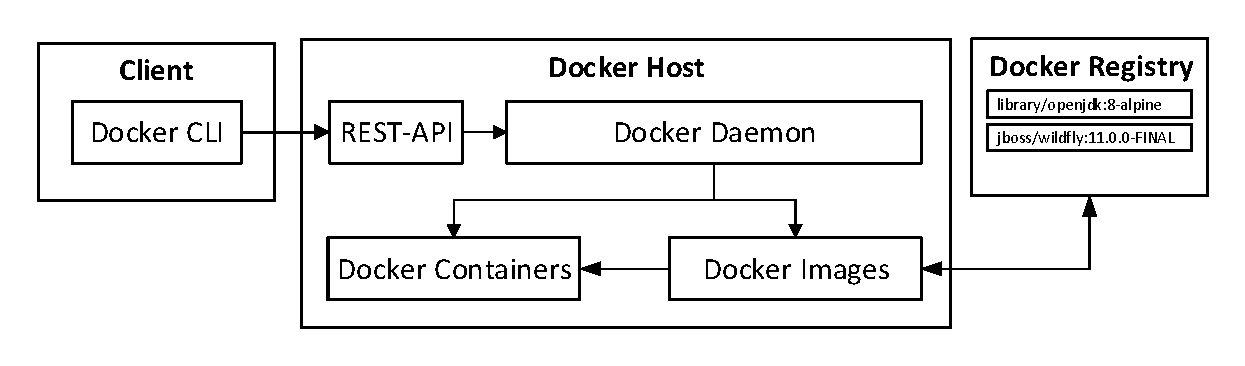
\includegraphics[scale=0.9]{images/docker-architecture.pdf}
	\caption{Docker Architecture}
	\label{fig:docker-architecture}
\end{figure} 

\subsection{Docker Machine}
\label{sec:docker-machine}
Docker Machine is a tool for managing local or remote Docker Hosts \cite{DockerMachine2018}. With Docker Machine an administrator can manage multiple Docker Hosts from a main server, without the need to connect to the Docker Host via secure shell (SSH). The Docker Machine CLI provides all commands necessary for managing Docker Hosts. Docker Engine provisions Docker Containers on a Docker Host and Docker Machine provisions Docker Hosts, in particular Docker Engines installed on docker Hosts. With Docker Machines a network of Docker Hosts can be managed, which is used by cloud platforms such as Openshift to manage Docker Engines on the nodes within the Openshift cluster.  

\section{Virtualization vs. Containerization}
\label{sec:docker-virtualization-vs-containerization}
Before LXC the industry made heavy use of operating system (OS) virtualization to isolate their environments and applications. A VM is managed by a Hypervisor, which is software, which can create, run and manage VMs. The VM provides resources such as network and storage for the application, which is managed by the virtualized OS. Nevertheless, an VM represents a full blown OS, which itself has a resource need which adds to the resource needs of the hosted application. LXC on the other hand are a kernel technology, which provides resources such as network and storage to the application as well, but without the need of virtualized OS.

\subsection{Virtual Machines}
\label{sec:docker-virtual-machines}
A Virtual Machine is an instance of a Virtual Machine Image (VMI), which is managed by a Virtual Machine Monitor (VMM), which is also referred to as the Hypervisor. The actual difference between a VMM and a Hypervisor is where the software is installed on. If the software is directly installed on the Hardware, then the software is called a Hypervisor, if its installed on the Host OS then its called a VMM. The VM abstracts  an Guest OS from the Host OS, in particular from the underlying hardware. A VM contained Guest OS is not bound to the underlying hardware, because the Hypervisor performs a kernel emulation, which allows to virtualize any Guest OS on any hardware, if the hypervisor supports it. The following Figure \ref{fig:docker-virtualization-architecture} illustrates the architecture of a virtualization system.

\begin{figure}[htbp]
	\centering
	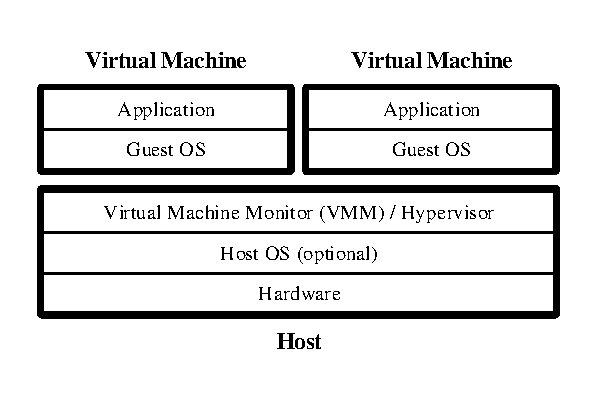
\includegraphics[scale=0.8]{images/docker-virtualization-architecture.pdf}
	\caption{Architecture of virtualized applications}
	\label{fig:docker-virtualization-architecture}
\end{figure} 

Glauber Costa's started the abstract of his talk at the LinuxCon 2012 with the humorous note \mentionedtext{"I once heard that Hypervisors are the living proof of operating system's incompetence"}. With this note he expressed that OS weren't able to provide proper isolation for applications and therefore the industry started to provide an OS instance for each application \cite{LxConCosta2012}. This has been overcome with the upcoming of LXC, which provide the proper isolation of applications on the same OS, which made the need for an OS instance for each application obsolete.

\subsection{Linux Container}
\label{sec:docker-linux-container}
The upcoming of LXC has eliminated the shortcoming to not be able to isolate applications properly of the Linux OS, which lead to using OS virtualization to isolate applications. LXC provide the feature of isolating applications running on the same OS, without the need of a kernel and hardware emulation as it is done with OS virtualization. As illustrated in Figure \ref{fig:docker-container-architecture}, the application process, binaries and libraries are bundled into the container and are isolated from other containers. Each container gets a portion o the global resources such as CPU cycles and memory assigned and cannot consume more as it has been assigned to. Without LXC it is possible that one process takes over the system resources and other processes get into state of starvation, which lead to need of OS virtualization. 

\begin{figure}[htbp]
	\centering
	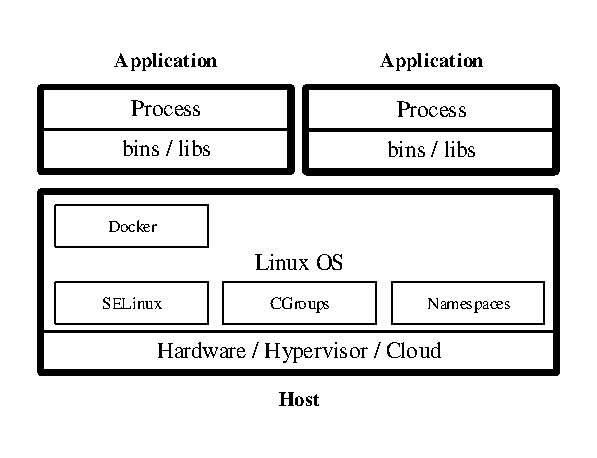
\includegraphics[scale=0.8]{images/docker-containerized-architecture.pdf}
	\caption{Architecture of containerized applications}
	\label{fig:docker-container-architecture}
\end{figure} 

The two most important kernel features underlying LXC are \mentionedtext{Cgroups} and \mentionedtext{Namespaces}. These two kernel features provide the resource control and isolation needed for application isolation and prevention of process starvation.

\mysubsubsection{Cgroups}
Cgroups stands for control groups and Cgroups provide the ability to aggregate processes, their child processes and threads within theses processes to groups managed in a tree structure. Each group gets a portion of the global resources such as CPU time, memory, I/O and network assigned, where its guaranteed that a group and its managed processes cannot consume more resources as the group has been assigned to. Each application hosted in a container is assigned to a group, where an application cannot steal resources from another application anymore, because the resource assignments of an group managed by Cgroups prevents this from happening \cite{KernelCGroupsV12018, KernelCGroupV22015, IntelLXCHyperVisor2014}. \\

\mysubsubsection{Namepsaces}
Cgroups manage how many resources can be used by processes in a group and namespaces manage the view of the system to processes. A container is managed in a namespace and therefore it has a limited view of the system such as networks and Process IDs (PIDs), depending on the configuration of the namespace the container is part of. Namespaces are a fundamental concept of LXC, and namespaces provide the isolation of a container \cite{LinuxNamespaces2018, IntelLXCHyperVisor2014}. \\

Docker has made the usage of LXC simple, but it is very hard to maintain a large set of Docker Containers (>100) via the Docker CLI, or to implement and maintain a cluster of Docker Hosts with Docker Machine. To much would have to be scripted manually, which would fast become very hard to maintain. Additionally, Docker does not provide any workflow for deployment and scaling of Docker Containers, and also does not ensure that a desired state of the containers is met. For a local development or a small set of containers the Docker CLI, Docker Compose and Docker Machine are suitable, but when it comes to large dynamic infrastructures with a large set of Docker Containers to maintain, then container orchestration platforms like Kubernetes, which is discussed in Chapter \vref{cha:caas}, will have to be used \cite{DockerSwarm2018, CNCFKubernetes2018}. 
 


\chapter{Container as a Service with Kubernetes}
\label{cha:caas}
Container as a Service (CaaS) is a term introduced by cloud providers, which provide a cloud based on demand container environment. But CaaS is more then just an on demand container environment like Docker, it provides orchestration and monitoring tooling for containers. Additionally, CaaS is considered to be a model for IT organizations and developers, how they can ship and run their applications anywhere. There are multiple CaaS providers on the market, but the most popular CaaS providers are Azure Container Service, Amazon Elastic Container Service for Kubernetes (Amazon EKS), and Google Kubernetes Engine, whereby they bring in their own flavor of CaaS, but all of them use Kubernetes beneath\cite{CNCFKubernetes2018, MicrosoftAzureAKS2018, AmazonWebServicesEKS2018, GoogleCloudKE2018}. \\

Kubernetes is a container orchestration platform for automating deployments, scaling, and operation of containers across a Kubernetes Cluster. Kubernetes has been invented by Google, is open source since 2015, and managed by the Cloud Native Computing Foundation (CNCF), whereby CNCF is under the umbrella of the Linux Foundation. Kubernetes has become the most popular container orchestration platform on the market and is used by many CaaS and PaaS providers\cite{CNCF2018}.

\section{The need for Container as a Service}
\label{sec:caas-need-for-caas}
Enterprises and developers face the need to dynamically adapt to workloads and to roll out new version of their services fast, and without any downtime. Applying dynamically to workloads requires a dynamic infrastructure, which is capable of scaling up when the workload increases, and scaling down when the workload decreases, which is non-trivial to be handled manually. Rolling out new versions without downtime require a well defined workflow, which ensures a well defined roll out behavior. For such uses cases, a CaaS platform like Kubernetes can be used. Kubernetes makes it possible to effortlessly manage complex service infrastructures, service scaling, and the roll out of services. Thus, complex service infrastructures become simple to implement and manage.
\newpage

Kubernetes provides a DSL, which allows to specify the desired state of the Kubernetes Cluster, as well as a automation tooling to interact with the Kubernetes Cluster. Kubernetes automatically ensures that the state of the Kubernetes Cluster meets its specification. Thus, the developers have only the need to specify the desired state of their Kubernetes Cluster. Kubernetes provides enterprises a platform for their services, which is effortlessly to specify and maintain via templates and the provided automation tooling, which makes Kubernetes an IaC tool as well, as discussed in Chapter \vref{cha:iac}. This makes it easy to modify the infrastructure at any time, which allows enterprises to apply to new requirements fast.

\section{Kubernetes}
\label{sec:caas-kubernetes}
Kubernetes is a CaaS platform to orchestrate containers in a cluster, whereby the Kubernetes Cluster nodes can be located in the cloud or in a dedicated data center. Kubernetes is designed as a client server architecture and a master slave architecture. At least one node in the Kubernetes Cluster acts as the Kubernetes Master, which is discussed in Section \vref{sec:caas-kubernetes-master}, and the other nodes in the Kubernetes Cluster act as the Kubernetes Workers, which are discussed in Section \vref{sec:caas-kubernetes-worker}. The Figure \ref{fig:kubernetes-cluster-architecture} illustrates the architecture of a Kubernetes Cluster.

\begin{figure}[htbp]
	\centering
	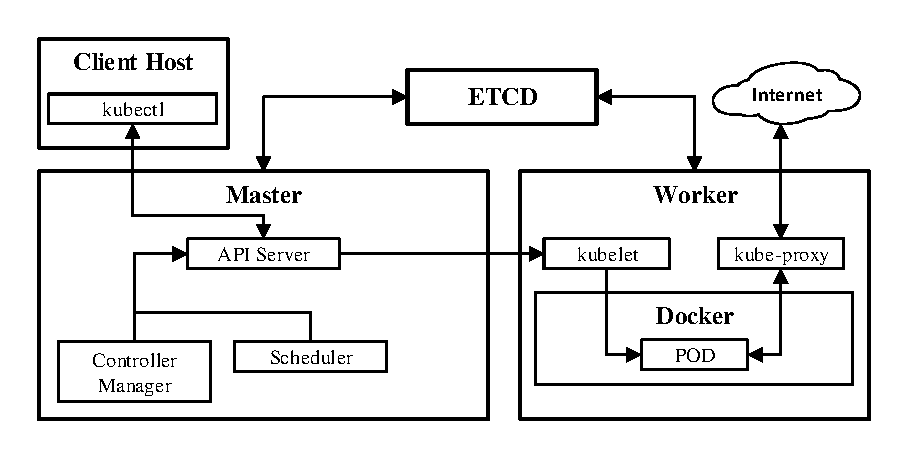
\includegraphics[scale=1]{images/kubernetes-cluster-architecture.pdf}
	\caption{Architecture of a Kubernetes Cluster}
	\label{fig:kubernetes-cluster-architecture}
\end{figure} 

\subsection{Kubernetes Objects}
\label{sec:caas-kubernetes-objects}
Kubernetes Objects are persistent objects in the Kubernetes System, and the Kubernetes Objects describe the state of the Kubernetes Cluster. The Kubernetes Cluster ensures that the state of the cluster meets the state specified by the Kubernetes Objects. The developers don't have to manually perform actions in the Kubernetes Cluster, they just have to modify the state represented by the Kubernetes Objects, and the Kubernetes Clusters itself will ensure that the modified state is applied on the Kubernetes Cluster. The following sections will briefly introduce some of the common used Kubernetes Objects. The overview of all Kubernetes Objects is covered by the Kubernetes API reference documentation\cite{CNCFKubernetesAPI2018}. 

\mysubsubsection{Pod}
A Pod is a group of one or more containers, which are managed together, and therefore share the same life-cycle. A Pod specification contains the specification for each container in the group. All of the containers of a Pod are always located on the same Kubernetes Worker, and will be deployed, started, and stopped as a single unit. In a pre-container world, all of the applications represented by the containers would have been hosted on the same physical machine. A Pod allows to bundle containers together, whereby the containers in a single Pod represent one instance of an  application\cite{CNCFKubernetesPods2018}. 

\mysubsubsection{Service}
A service is an abstraction, which defines a set of Pods and policies how to access them. The connection to the Pod, via the service abstraction, is handled by the Kubernetes Proxy. The service abstraction is necessary, because a Pod can be located on any Kubernetes Worker within the Kubernetes Cluster, and the Pod will therefore get a random IP assigned, which makes it impossible to address the Pod directly. If multiple replicas of a Pod are running, then the service will load balance the request between the Pods of the replica set, depending on the chosen algorithm\cite{CNCFKubernetesServices2018}.

\mysubsubsection{Secret}
A secret is an abstraction to manage sensitive configuration data, which can be consumed by containers. A secret holds a set of key value pairs, which represents the sensitive configuration data, and can be referenced by its name. A referenced secret can be injected into the container, either as a environment variable or a file. If the secret is injected as a file, then the filename represents the secret key and the file content represents the secret value. Developers reference secrets in the Pod specifications by their name, and only the referencing containers can access the injected sensitive configuration data the secret holds\cite{CNCFKubernetesSecrets2018}. 

\mysubsubsection{ConfigMap}
A configuration map works the same way as secrets, but is intended to hold non sensitive configuration data\cite{CNCFKubernetesConfigMap2018}.

\subsection{Kubernetes Master}
\label{sec:caas-kubernetes-master}
The Kubernetes Master is the master node in the Kubernetes Cluster, and is responsible for managing the Kubernetes Workers and Pods running on them. The Kubernetes Master exposes a REST API, via clients can interact with the Kubernetes Cluster. The node hosting the Kubernetes Master should be exclusively for the Kubernetes Master. The following sections briefly introduce the Kubernetes Master-Components, which are responsible for managing the Kubernetes Cluster\cite{CNCFKubernetesComponents2018}.

\mysubsubsection{Kubernetes CLI (kubectl)}
Kubectl is the CLI of Kubernetes, which provides an interface to manage the Kubernetes Cluster, and the Pods running on the Kubernetes Workers. Kubectl is similar to the Docker CLI, but does not support direct interacting with Docker. Kubectl interacts with the Kubernetes Cluster via the REST API exposed by the Kubernetes Master API-Server. Kubectl can be used from any client machine, which can connect to the cluster without any special setup.

\mysubsubsection{Distributed Key-Value Store (etcd)}
Etcd is a distributed key-value store, and provides a reliable way for sharing data within a cluster. It is the key component for the communication between the Kubernetes Masters and the Kubernetes Workers. The Kubernetes Master provides configuration for the Kubernetes Workers, and the Kubernetes Workers provide state information for the Kubernetes Master\cite{CoreOSETCD2018}.

\mysubsubsection{Kubernetes API-Server (kube-apiserver)}
The Kubernetes API-Server exposes the REST API for interacting with the Kubernetes Cluster, and is located on the Kubernetes Master. It represents the front-end of the Kubernetes Cluster and provides all necessary API to manage the Kubernetes Cluster, and the Kubernetes Objects.

\mysubsubsection{Kubernetes Scheduler (kube-scheduler)}
The Kubernetes Scheduler watches the Kubernetes Cluster for newly created Pods and assigns the Pods to a Kubernetes Worker. The Kubernetes Scheduler decides which Kubernetes Worker is suitable for the Pod. Multiple factors are taken into account for scheduling decisions such as, individual specifications, resource requirements, available resources, and hardware/policy/software constraints.

\mysubsubsection{Kubernetes Controller Manager (kube-controller-manager)}
The Kubernetes Controller Manager is responsible for managing the different controllers. A Kubernetes Controller is running in a loop and ensures that the state of the system is valid, depending on the controller type. For instance, the replication controller ensures the correct number of Pods for each replication controller object within the Kubernetes Cluster. Kubernetes provides a set of controllers such as, a replication controller, node controller, endpoint controller, and service account controller.

\subsection{Kubernetes Worker}
\label{sec:caas-kubernetes-worker}
The Kubernetes Worker is a node within the Kubernetes Cluster, which acts as the slave node, which runs the Pods, and is managed by the Kubernetes Master. The Kubernetes Worker can be a VM or a physical machine, depending on the Kubernetes Cluster setup. It contains the Kubernetes Runtime-Environment and used container runtime. The following sections briefly introduce the Kubernetes Worker-Components, which are responsible for running the Pods on the Kubernetes Worker\cite{CNCFKubernetesComponents2018}. 

\mysubsubsection{Kubernetes Agent (kubelet)}
The Kubernetes Agent is a process, running on the Kubernetes Worker, which interacts with the Kubernetes Master via its exposed REST API. The Kubernetes Agent ensures, that the containers are running in a Pod, as specified by the provided Pod specifications. The Pod specifications can be provided by a file in a specific directory, which gets periodically checked, or via the Kubernetes API-Server.

\mysubsubsection{Kubernetes Network-Proxy (kube-proxy)}
The Kubernetes Network-Proxy manages the networks defined by the specifications, and reflects the services, which are bound to a Pod. It can perform simple TCP and UDP forwarding, and can be connected to multiple back-ends. Any communication of a Pod to another Pod or to an external network is handled by the Kubernetes Network-Proxy. 

\mysubsubsection{Container Runtime}
The container runtime is the software responsible for running the containers on the Kubernetes Worker. Kubernetes supports multiple container runtimes, but mostly  Docker is used, which has been discussed in Chapter \vref{cha:containerization-docker}. \\

Kubernetes provides all features to implement a dynamic scalable service infrastructure such as, workflows for rolling out services, replica management, or secret and configuration management. Kubernetes is on top of the container runtime such as Docker, and provides orchestration tooling, necessary to run large scale containerized service infrastructures. Nevertheless, sometimes a pure container orchestration platform like Kubernetes is not enough, which for instances doesn't provides features for setting up a complete release workflow. This can be overcome with the usage of PaaS platforms like Openshift, which will be discussed in the following chapter.

\chapter{Platform as a Service with Openshift}
\label{cha:paas}
Platform as a Service (PaaS) ...

\section{The need for Platform as a Service}
\label{sec:paas-need-for-paas}

\section{Openshift}
\label{sec:paas-kubernetes}
\chapter{Enterprise Service Bus}
\label{cha:esb}
An Enterprise Service Bus (ESB) is a architectural pattern which describes a distributed computing architecture, whereby distributed services are interacting with each other via the ESB. The ESB pattern if part of the Service Oriented Architecture Patterns (SOA).   
\\ \\
An ESB in the industry is mostly taken as a third party middleware, which provides features for implementing integrations with the Enterprise Integration Patterns (EI). Enterprises use third party middleware like JBoss Fuse for implementing integration services, which integrate external or internal services. JBoss Fuse is based on the Enterprise Application Platform (EAP), and bundles common frameworks used for integrations such as Camel, and is responsible for orchestration and mediation of the services.
\\ \\
The integration of internal as well as external services has become more important over time, especially with the appearance of cloud platforms like PaaS. Common ESB middleware on the market usually define the ESB as a single application, which contains all integration services, whereby all integration services share the same life-cycle. But the need for flexibility and shorter response times drives enterprises to split up their teams and integrations. This leads to separated services, which are managed as microservices, which have their own life cycle. De-coupling of teams leads to de-coupling of services, where the services need to provide a well defined and well managed public API\cite{Camel2015, RedHatAgileIntegration2017, EIP}.

\section{The need for an Enterprise Service Bus}
\label{sec:esb-need-for-esb}
Enterprises need an ESB to provide integrations between internal and external services or both, where the integration is meant to provide a business value for the enterprise. An integration of an external service could enhance the reach of a customer, who now could be able to consume external partner services via the enterprise provided infrastructure or product. In the digital age, it is normal to consume a digital service like Netflix, which runs a streaming service. Thus, integrations an enterprise has to provide and maintain will become more over time.

\section{Architecture}
\label{sec:esb-architecture}
Figure \vref{fig:esb-simple-architecture} illustrates the conceptional architecture of an ESB, which orchestrates and mediates integration services. A service can act either a producer service, which gets accessed by clients, or can act as a consumer service, which acts as the client for a producer service. The ESB is responsible for orchestration, mediation, security, transformation, routing and service discovery, whereby these aspects are covered by a ESB middleware provided frameworks and libraries. Additionally, an ESB middleware provides libraries which help to implement Service Components under consideration of the SOA and EI Patterns\cite{EsbSoa2018, MediationESB2005}.

\begin{figure}[htbp]
	\centering
	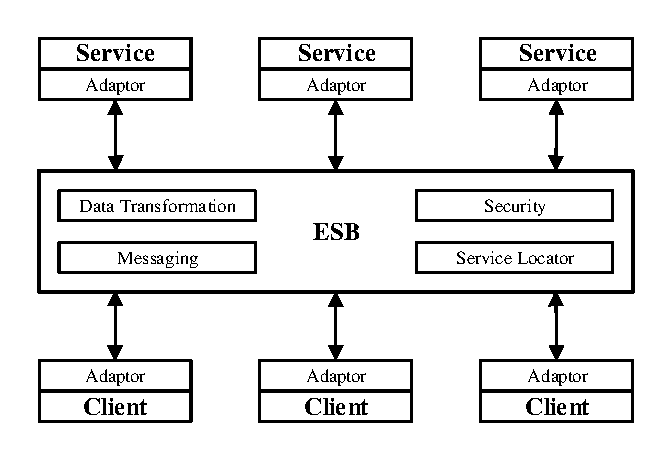
\includegraphics[scale=1]{images/esb-simple-architecture.pdf}
	\caption{Architecture of an ESB}
	\label{fig:esb-simple-architecture}
\end{figure} 

\begin{figure}[htbp]
	\centering
	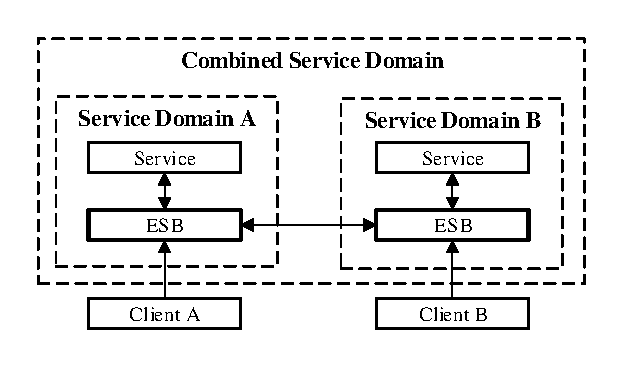
\includegraphics[scale=1]{images/esb-bidirectional-integration.pdf}
	\caption{Architecture of a bi-directional enterprise integration}
	\label{fig:esb-bidirectional-integration}
\end{figure} 

Figure \vref{fig:esb-bidirectional-integration} illustrates a bi-directional integration of services between two partner enterprises, whereby each integrated service is allowed to be consumed by the partner's customers, but only if the service is accessed via the partner's infrastructure. The ESB of the enterprises integrate the partner's provided services into their service domain, which can be accessed by their customers. For instance, an IP-TV provider can be integrated by an Internet Service-Provider (ISP), to provide Internet TV to their customers. 

\section{ESB with EAP}
\label{sec:esb-as-software}
An ESB is an architectural pattern for a distributed system, and has been implemented in software to provide an integration platform to developers, so that they can implement services under the consideration of the EAI patterns. Before the appearance of cloud platforms like PaaS, ESB implementations used existing platforms such as JBoss EAP, OSGI or Karaf for the service orchestration and mediation. In case of JBoss EAP, the platform provides all libraries and frameworks developers need for implementing a service. Commonly, the services are managed within a single application, which represents ESB. This is a monolithic approach of organizing services, but has the advantage that the management of the services is easier, because the source code is not separated, and therefore the implementations of all services needs to be consistent at compile time. Figure \vref{fig:esb-software-architecture} illustrates the monolithic organization of the services within a single ESB application, which is hosted on JBoss EAP.

\begin{figure}[htbp]
	\centering
	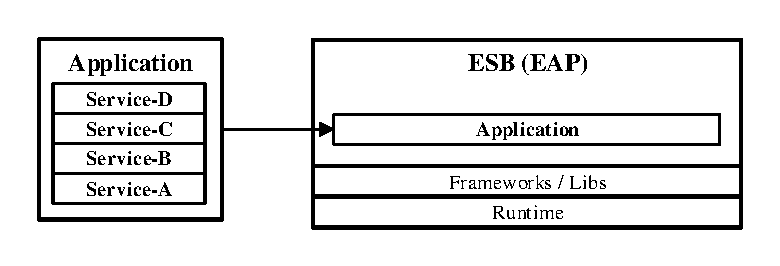
\includegraphics[scale=1]{images/esb-software-architecture.pdf}
	\caption{ESB running on EAP}
	\label{fig:esb-software-architecture}
\end{figure} 

With the appearance of cloud platforms such as PaaS, the cloud can now take over the mediation, orchestration and security aspects of an ESB. The integration services can be completely separated and de-coupled from each other, designed as microservices with their own life-cycle, and be managed by the cloud platform. Additionally, the integration services are hosted in a clustered infrastructure, which allows them to be distributed among multiple nodes, which increases fail over security. The new term for this kind of ESB is IPaaS, whereby the ESB is represented by an PaaS platform such as Openshift, which provides additional tooling for implementing integration services\cite{iPaaSP12015, iPaaSP22015}.

\section{ESB with Openshift}
\label{sec:esb-as-cloud}
With the appearance and general availability of cloud platforms like PaaS, it is possible now to move an ESB into the cloud, whereby the cloud platform takes over some aspects of the ESB middleware such as mediation and orchestration. A main problem of existing ESB implementations is the fact, that all integration services are managed within a single application, with one release version, and a shared life-cycle. If the ESB is an cloud platform, the integration services have to be implemented as separated services, which forces developers to separate their integration services into separate code bases, and to provide a proper designed and managed public API for their services. Figure \vref{fig:esb-cloud-architecture} illustrates the integration services of an ESB application, which runs on Openshift.

\begin{figure}[htbp]
	\centering
	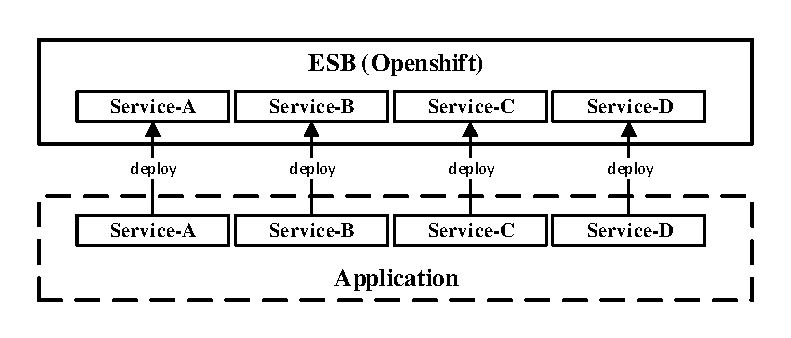
\includegraphics[scale=1]{images/esb-cloud-architecture.pdf}
	\caption{ESB application architecture with microservices}
	\label{fig:esb-cloud-architecture}
\end{figure} 

As discussed in the introduction of this chapter, enterprises need to separate their integrations and teams, to be faster and more responsive to business changes. Therefore, the microservice architecture, which is necessary when the ESB is represented by a cloud platform, can help enterprises to become more flexible.

\section{Integration example}
\label{sec:esb-integration-example}
This section will discuss an integration examples, and how it would have been designed as part of a monolithic ESB application. The integration discussed in this chapter is the base for the prototype of this thesis, which is specified in Chapter \vref{cha:esboc}. Figure \vref{fig:esb-design-services} illustrates the integration example, contained services and involved service domains. The integration service integrates an external database with an internal application, which is consumed by a public client. How the database is allowed to be accessed, is implemented in the integration service, which is the only service allowed to communicate with the external located database.
\newpage

\begin{figure}[htbp]
	\centering
	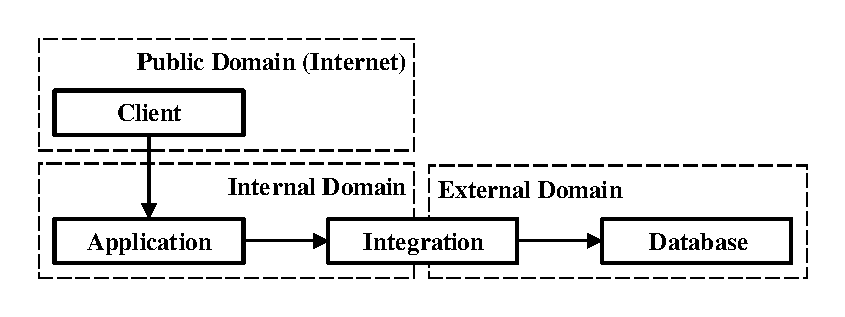
\includegraphics[scale=1]{images/esb-integration-example.pdf}
	\caption{Integration Service-Domains}
	\label{fig:esb-design-services}
\end{figure}

Figure \vref{fig:esb-design-sca} illustrates the design of the integration in an monolithic ESB application, with the use of Service Component Architecture (SCA). A service within the ESB application is represented by a service component, which exposes consumable services (\mentionedtext{Service}) and is connected to other services or external systems (\mentionedtext{Reference}). 

\begin{figure}[htbp]
	\centering
	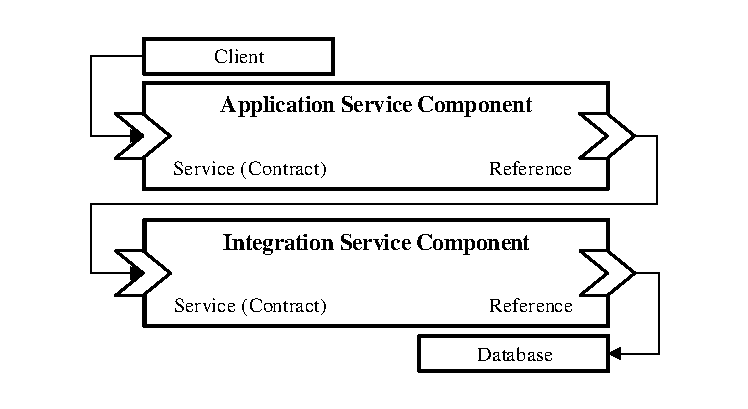
\includegraphics[scale=1]{images/esb-sca-example.pdf}
	\caption{Integration Services with SCA}
	\label{fig:esb-design-sca}
\end{figure}
  
ESB middleware, such as JBoss Fuse provides frameworks and libraries, which implement the SCA patterns and provide a lightweight way of implementing service components. The service component orchestration, mediation is done by the ESB middleware. Additionally, the ESB middleware provides bindings for commonly used technologies such as REST or SOAP, which can be applied to services and references. Thus, the developers don't have to setup for instance a REST Server or REST Client anymore, but only need to provide the service contract and connection settings\cite{MicroSoa2008, Richards2015}.\\

The following chapter will specify the prototype based on the introduced integration example, and will show that an ESB can be implemented on Openshift.
\chapter{Design ESB in Openshift}
\label{cha:esboc}
As discussed in Chapter \vref{cha:esb}, an ESB is a distributed computing architecture, where distributed services act as a consumer or producer. These services provide a business value in form of an integration of an internal or external service for an enterprise. There are multiple providers of ESB middleware like JBoss Fuse, as discussed in Section \vref{sec:esb-middleware}, which provide tooling for implementing service components hosted on an ESB. It should be possible to migrate such a service component to a microservice, where features provided by the ESB middleware will have to be replaced by other implementations.
\\ \\
In this chapter an ESB application will be designed, where a service and a database will be integrated into each other by a another service. An Openshift Project will represent the service bus, which hosts the integration service, provides configuration and manages secrets for it. The concrete implementation of the services is considered to be not important, because they services will be ordinary Java web applications, which are known to be able to consume frameworks used in the Java Enterprise field. More important is the concept of how to represent a service component of an ESB as a microservice and how to host such microservices in Openshift which acts as the actual service bus.

\section{Service Architecture}
The Figure \vref{fig:esboc-design-services} illustrates the concept of the service architecture. This service architecture acts as an example of an application integration on an ESB. In an real world example such an service architecture would only represent a fraction of the actual services hosted on the ESB, which leads to the question how such an ESB can be monitored, especially when the integration services are hosted as separate microservices? The prototype will address the need for monitoring of the microservices by implementing tracing and logging features, which are discussed in Section \vref{sec:esboc-requirements-service}.

\begin{figure}[htbp]
	\centering
	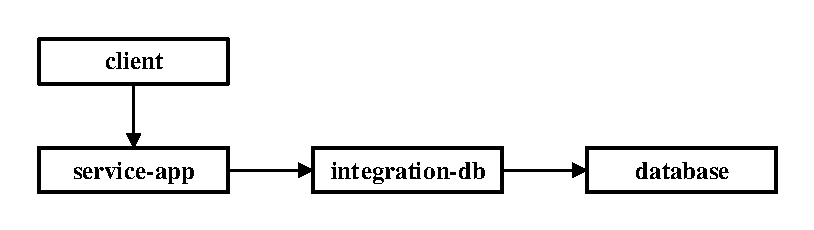
\includegraphics[scale=1]{images/esboc-design-services.pdf}
	\caption{Service Architecture}
	\label{fig:esboc-design-services}
\end{figure}

\subsection{Client}
\label{sec:esboc-design-service-client}
The client will be a Java REST-Client which consumes data from the backing service application. The REST-Client could be a single page web application or an other back-end application. It will have no direct access to the database or the integration service, which integrates the database and the Service application, and is therefore completely abstracted of the underlying data storage and its schema.

\subsection{Service Application}
\label{sec:esboc-design-service-app}
The service application act as the back-end service for the client and produces data consumed by the client. The service application consumes from the integration service, which acts as the its back-end service. Same as the client, the service application is abstracted of the underlying data storage and its schema. 

\subsection{Integration Service}
\label{sec:esboc-design-service-integration}
The integration service acts as the front-end service of the database and the back-end service for the consumers. The integration service ensures that the consumers are abstracted of the underlying data storage and its schema, as well as that the database is accessed in a proper manner, by providing a public API which defines the operations and models.

\subsection{Database}
\label{sec:esboc-design-service-database}
The database acts as the data source for client which indirectly access this database via the integration service or a back-end service which itself is backed by the integration service. This level of abstraction of the consumers allows the database to evolve decoupled from the actual consumers. There is only the integration service which would have to be modified, when the underlying database or its schema changes.
\newpage

\section{Service Requirements}
\label{sec:esboc-requirements-service}
In this section the service requirements will be specified, which will ensure that the services are properly implemented and can effortlessly be managed and monitored. Especially the management and monitoring becomes very important when moving from a conventional ESB application, like an application running on JBoss Fuse, to a microservice architecture, which is hosted on a PaaS platform like Openshift. Hosted on Openshift, the services run completely decoupled from each other with their own life cycle, which makes the management and monitoring harder compared to manage and monitor a monolithic application.

\begin{figure}[htbp]
	\centering
	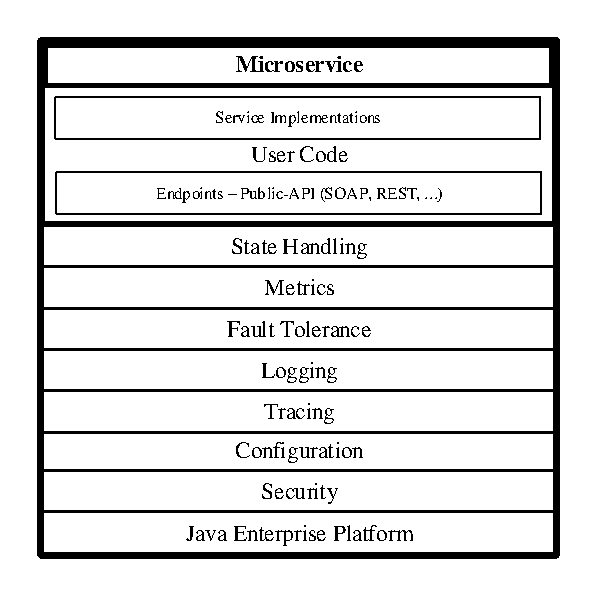
\includegraphics[scale=1]{images/esboc-requirement-services.pdf}
	\caption{Service Requirements}
	\label{fig:esboc-requirements-services}
\end{figure} 
Figure \vref{fig:esboc-requirements-services} illustrates the hierarchy of the service requirements, represented by the layers below the \mentionedtext{User Code} layer. The service requirements, which are specified in the following sections, will ensure that the microservices are
\begin{itemize}
	\item secure,
	\item configurable for multiple environments
	\item observable by developers and operators,
	\item resilient to failures
	\item and measurable.
\end{itemize}

\subsection{Technology}
\label{sec:esboc-requirements-service-technology}
The services will be implemented in Java with the Java Enterprise Platform and the MicroProfile specifications. The MicroProfile specifications are an effort of the Eclipse Foundation to make Java applications ready for the cloud, where especially monitoring is a very important aspect to consider when it comes to distributed services. The services will be hosted as standalone applications like Spring Boot applications \cite{EclipseMicroprofileCharter2017, EclipseEE4JCharter2017}.

\subsection{Security}
\label{sec:esboc-requirements-service-security}
The integration service will be secured with OAuth to protect its exposed endpoints from unauthorized access. OAuth is a token based authentication scheme, which has become popular over past few years. The  integration service must authenticate its client the service application against an central authentication service, whereby the the service application will retrieve the access tokens from the central authentication service \cite{OAuth2018}.

\subsection{Configuration}
\label{sec:esboc-requirements-service-config}
The MicroProfile specifications provide the MicroProfile-Config specification, which provides an API to inject configuration parameters into classes, which can be loaded from different configuration sources. The services must provide the possibility to be configurable for different stages such as DEV (development), TEST (testing) and PROD (productive environment), where the services must not directly access the configuration sources, or hard code configuration in the source code unless its a default parameter \cite{EclipseMicroprofileConfig2018}.

\subsection{Monitoring}
\label{sec:esboc-requirements-service-monitoring}
Monitoring is a essential aspect in distributed service architecture. Operators and developers need logging and tracing information of the services to comprehend errors in the services, where the cause of a problem could be located at another service as the service where a problem is reported.

\mysubsubsection{Distributed Tracing}
Distributed Tracing allows to comprehend service or method call chains. The MicroProfile specifications provides the OpenTracing specification, which provides an API for tracing an application on a method level or across service boundaries. The services must be able to collect tracing information about the REST and the related service method calls, and send this data to a central tracing service. The tracing implementation must be implemented separately from the service logic \cite{CNCFOpentracing2018}.

\mysubsubsection{Distributed Logging}
Distributed Logging allows to comprehend logs across service boundaries within a service call chain, where the logs of a service call chain have to be marked with a transaction id. The services must be able to provide all of their logging to a central service, whereby the logs are marked with a transaction id, which is equivalent to the transaction id of the service tracing. Optionally the services are allowed to add additional markers, which can help developers and operators to analyze problems or to group service logs.

\subsection{Fault Tolerance}
\label{sec:esboc-requirements-service-fault}
The MicroProfile specifications provide the specification MicroProfile-Fault-Tolerance, which provides an API to define fault tolerance behavior such as retries, timeouts and error fall-backs. The fault tolerance of a service means that, if a depending service is not accessible at the time, a service must not fail immediately after the first try, but the service should retry to call the depending service for several times, and fail when all retries have failed. Such a behavior ensures that short timed communication errors, redeployments or overloads do not immediately cause a service to fail. The services must provide proper fault tolerance configuration and fall-back behavior to be able to recover from such errors in a proper manner. \cite{EclipseMicroprofileFault2018}.   

\subsection{State Handling}
\label{sec:esboc-requirements-service-state}
The service will be stateless, so that the services can be scaled and any request be handled by any instance of the service. Additionally Blue-Green-Releases and Canary-Releases are easily possible with stateless services \cite{FowlerBlueGreenRelease2010, FowlerCanaryRelease2010}. Multiple instances of stateful service hosted on a PaaS platform are not flexible as stateless services, because sessions must stick to a particular service instance, and persistence volumes have to be shared between the service instances.  

\subsection{API Management}
\label{sec:esboc-requirements-service-api}
The API management of a public API such as REST-API REST-Models ensure that the clients, using a public API, are not broken by changes made on that API. There are several opinions on how API management can be done. Swagger has become very popular for documenting REST-API, where the documentation can be used to generate clients, provide documentation for developers and to test the public API. The services must be capable of migrating their public API in a way that the clients are not broken by the change. The replaced API version must be supported as well as the new one, so that the client is not forced to modify its source code \cite{SmartBearSwagger2018}.

\textbf{ADD resource which christoph found during liwestfsw research} 
\section{Openshift Architecture}
\label{sec:esboc-design-oc}
Figure \vref{fig:esboc-design-openshift-project} illustrates the structure of the Openshift Project, as well as the service dependencies within the Openshift Project. As discussed in Section \vref{sec:paas-openshift}, Openshift isolates the namespaces, which are representing an Openshift Project. Therefore, the services within this Openshift Project, which are not exposed via an Openshift Route, are implicitly protected from external access from the Internet or services hosted in another Openshift Projects. The Openshift Project contains the service application, the database and the integration service, whereby the service application and the database would normally be located outside the Openshift Cluster. The service application has access to the Internet and will be accessed by the client from the Internet via its public address. The integration service and the database are not exposed to the Internet and can only be accessed within the Openshift Project by their service names.

\begin{figure}[htbp]
	\centering
	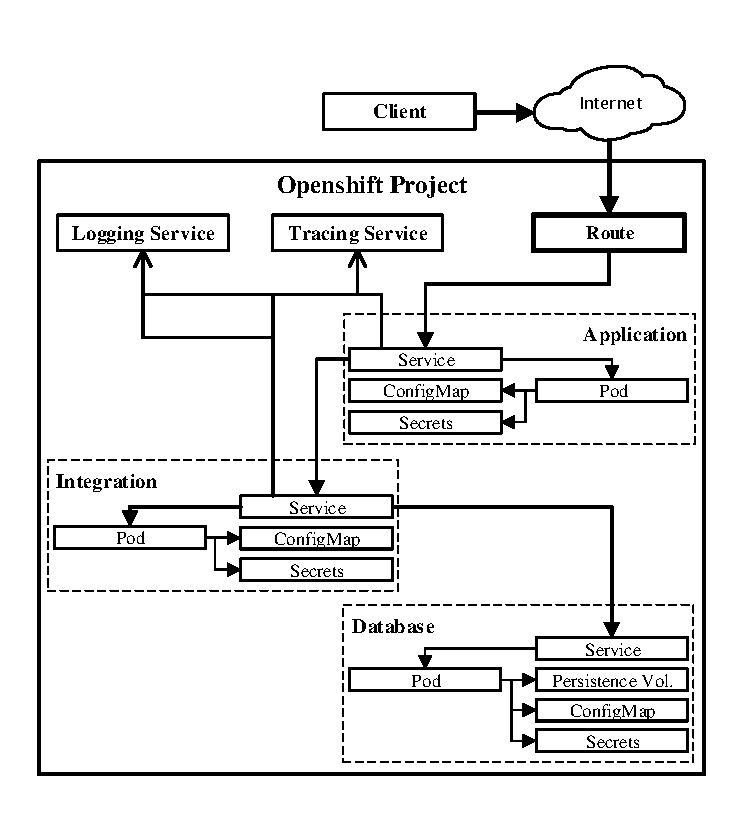
\includegraphics[scale=1]{images/esboc-design-openshift.pdf}
	\caption{Openshift Project architecture}
	\label{fig:esboc-design-openshift-project}
\end{figure} 

\section{Openshift Requirements}
\label{sec:esboc-requirements-oc}
The implementation of the Openshift resources such as templates and scripts must be implemented under consideration of the principles of IaC, as discussed in Section \vref{sec:iac-principles}. Keeping to the principles of IaC will ensure, that the Openshift Project can effortlessly be recreated with a different configurations for the intended stages. This allows the developer for instance to implement integration tests, where service dependencies such as the database can be mocked or be replaced by a test database.

\subsection{Openshift Project}
\label{sec:esboc-requirements-oc-project}
The Openshift Project will not only host the services, but will manages their configuration and secrets, which have been discussed in Section \vref{sec:caas-kubernetes-objects}. The separation of the service implementation from the configuration as well as the secrets, ensures that the configurations and secrets can be applied on a service without a new release, and that developers do not have to handle secrets anymore, which increases the security.

\subsection{Monitoring}
\label{sec:esboc-requirements-oc-monitoring}
To be able to monitor the hosted services, the Openshift project must host two monitoring services, one for log aggregation, and another one for tracing aggregation. In a real world example, the log aggregation and tracing services would be located in another Openshift Project or outside the Openshift Cluster. 

\chapter{Implementation ESB in Openshift}
\label{cha:esbi}
This chapter will discuss the implemented prototype, which has been designed in Chapter \vref{cha:esboc}. The implemented prototype uses a lot of technologies and specifications, which are beyond the scope of tis thesis, therefore this thesis will focus on the most important implementation parts. A focus will be set on the implementation of the aspects discussed in Section \vref{sec:esboc-aspects}, which ensure that a integration service can be managed properly in a Openshift Cluster. 
\\ \\
The integration services are implemented as microservice, which run as standalone applications on the Openshift Cluster, with their own life cycle. The integration services communicate via REST with each other, whereby each service provides a proper managed public API. The code bases of the integration services are managed separately, which completely de-couples the integration service from each other.  
\\ \\
As the prototype illustrates, the ESB is now represented by Openshift, which acts as the platform for the hosted integration services. The hosted integration services are implemented as microservices and are running in Docker Containers as standalone applications. Horizontal scaling and the distribution of the services over multiple hosts are now possible. Section \vref{sec:esbi-openshift} will discuss the implemented Openshift resources, which are used to define and manage the Openshift Project.
\\ \\
Is is assumed, that the reader is familiar with Java Enterprise Development, Maven and microservices. The implemented prototype is available on Github \footnote{https://github.com/cchet-thesis-msc/prototype}. The repository contains a README file, which describes how to setup the prototype. 

\section{Microservice Technologies}
\label{sec:esbi-technolody-fis}
The following sections will give a brief introduction about the most important technologies used to implement the integration services. Each implemented service uses the same technologies and is build the same way, because no matter what the concrete purpose of the service is, they all have to be integrated and run the same way on a Openshift Cluster.

\subsection{JBoss Fuse Integration Services 2.0}
\label{sec:esbi-technology-fis}
JBoss Fuse Integration Services 2.0 is a set of tooling for developing integration services running on a Openshift Cluster. It provides Openshift integrations for different frameworks such as Spring Boot, Karaf or Camel. The services are started via an Java-Agent such as Prometheus or Jolokia, which are used to monitor the service during runtime. Additionally to provided Openshift resources, a Maven Plugin is provided, which allows to interact with the Openshift Cluster during a Maven build. JBoss Fuse Integration Services 2.0 allows developers to interact with a Openshift Cluster in a way like developers did before with an application server \cite{Prometheus2018, Jolokia2018}.

\subsection{Wildfly Swarm}
\label{sec:esbi-technology-swarm}
Wildly Swarm is the JEE answer to Spring Boot, and is a framework, which allows to package an application into an Uber-JAR. An Uber-JAR is a packaged standalone application, which can be started with the command \inlineJava{java -jar}. During the packaging, only those components of an application server are packaged, which are referenced and needed by the application. The application can then be started via \inlineBash{java -jar app.jar}, whereby the application server is bootstrapped programmatically.  The application deployment artifact is a JAVA Web-Archive, which could be hosted in any application server environment, which provides all of the referenced dependencies \cite{WildflySwarm2018}. 

\subsection{Fabric8}
\label{sec:esbi-technology-f8}
Fabric8 is an integrated development platform for developing applications on Kubernetes. Fabric8 provides the Maven Plugin for the JBoss Fuse Integration Services 2.0, and focuses on building Docker Images, managing Kubernetes or Openshift resources and deploying Java applications on Kubernetes or Openshift Clusters \cite{Fabric82018}.
\\ \\
The next Section will discuss the implementations of the microservice aspects discussed in Section \vref{sec:esboc-aspects}.

\section{Security}
\label{sec:esbi-security}
The integration services are secured with OAuth, and authenticate their clients via Keycloak. Keycloak is used as the authentication service, and is a very popular open source identity and authentication application. Wildfly Swarm provides an integration into Keycloak via the Keycloak-Adapter, which only needs to be added as a dependency to the Maven POM and to be configured.

\subsection{Service}
\label{sec:esbi-security-service}
This section will discuss the implementation of the security in the service implementations. Listing \vref{ls:esboi-security-pom} shows the dependency, which brings in the Keycloak Adapter, integrates itself into the Java Web-Security mechanisms, and can therefore be configured with Java Web-Security security constraints.
\begin{listing}
	\xmlFile{\sourceDir/maven-keycloak-swarm.xml}
	\caption{Wildfly Swarm Keycloak dependency in pom.xml}
	\label{ls:esboi-security-pom}
\end{listing}

Listing \vref{ls:esboi-security-yaml} shows an excerpt of the Wildfly Swarm configuration file project-stages.yml, which configures the security constraints for the REST-Endpoint.

\begin{listing}
	\yamlFile{\sourceDir/project-stages-security.yml}
	\caption{Security configuration in project-stages.yml}
	\label{ls:esboi-security-yaml}
\end{listing}

The following two listings are excerpts of the deployment.yml Openshift Template, which is managed in the service code base. Listing \vref{ls:esboi-security-oc-deployment-volume-secret} shows the specification of the secret injection into a Docker Volume. The secrets are injected as files, whereby the file name represents the secret key and the file content represents the secret value. Therefore, that the secrets are managed externally, the developers need to provide the secret name for the service deployment configuration. In this case an expression is used, which can be replaced by Maven Properties, whereby the Maven Properties can be provided in the pom.xml or provided/overwritten by Java Options, during the build process.

\begin{listing}
	\yamlFile{\sourceDir/deployment-volume-secret.yml}
	\caption{Configuration of the secret injection}
	\label{ls:esboi-security-oc-deployment-volume-secret}
\end{listing}

Listing \vref{ls:esboi-security-oc-deployment-volume-mount} show the specification of the mount of the Docker Volume, which provides the secrets. The mount path is also represented by a Maven Property, because this path is also used in the project-stages.yml file, where it points to the service configuration source for the productive stage. The secrets consumed by the services are used the same way as non-sensitive configurations, which are discussed in Section \vref{sec:esbi-configuration}.

\begin{listing}
	\yamlFile{\sourceDir/deployment-volume-secret-container.yml}
	\caption{Configuration volume mount}
	\label{ls:esboi-security-oc-deployment-volume-mount}
\end{listing}

\subsection{Openshift}
\label{sec:esbi-security-openshift}
This section will discuss the Openshift implementation, whereby the implementation is represented by a shell script, which manages the secrets. The secrets are managed outside the code bases of the integration services.
\\ \\
Listing \vref{ls:esboi-security-oc-secret} shows the Openshift CLI-Commands, which are used to create the secrets. The first command creates a secret from literal values which is used by a client service to retrieve authentication tokens. The second command creates a secret from a file, whereby the filename is the secret key and the content is the secret value, which is used by the Keycloak Adapter to validate authentication tokens provided by the clients. 

\begin{listing}
	\bashFile{\sourceDir/bash-oc-secret.txt}
	\caption{Openshift CLI command for creating the secret}
	\label{ls:esboi-security-oc-secret}
\end{listing}

The discussed implementations are the necessary implementations on the Service and Openshift side, to secure services hosted on a Openshift Cluster. No infrastructure code is necessary, only configuration. The following section will discuss the configuration of the integration services, which can be applied to the security as well, because secrets in Openshift are used in the service implementations the same way as configuration parameters.

\section{Configuration}
\label{sec:esbi-configuration}
The integration services use the MicroProfile Config specification to be configurable for multiple stages by exposing all necessary configuration parameters and to be able to consume configuration parameters from different configuration sources via injection. Developers are bound to the configuration or secret name, keys and their value type, but developers are not bound to the configuration or secret source, which allows to provide configurations from different sources and for different stages. 

\subsection{Service}
\label{sec:esbi-config-service}
This section will discuss the implementation of the configuration definition and usage. Listing \vref{ls:esboi-config-pom} shows the dependency, which brings in the MicroProfile Config specification to enable injectable configurations.
 
\begin{listing}
	\xmlFile{\sourceDir/maven-microprofile-config.xml}
	\caption{Wildfly Swarm MicroProfile-Config dependency in pom.xml}
	\label{ls:esboi-config-pom}
\end{listing}

Listing \vref{ls:esboi-config-project-stages-dev} shows the definition of the configuration source with the name \mentionedtext{app.secrets} for the development stage, whereby the configuration properties are provided hard coded.

\begin{listing}
	\bashFile{\sourceDir/project-stages-micro-config-dev.yml}
	\caption{Hard coded configuration for development stage}
	\label{ls:esboi-config-project-stages-dev}
\end{listing}

Listing \vref{ls:esboi-config-project-stages-prod} shows the definition of the configuration source with the name \mentionedtext{app.secrets} for the production stage, whereby the configurations are loaded via a directory. The directory location is represented by an Maven Property, because its used in multiple configuration files, as already discussed in Section \vref{sec:esbi-security-service}. The MicroProfile Config specification will load files in this directory by using the filename as the key and the content as the value.

\begin{listing}
	\yamlFile{\sourceDir/project-stages-micro-config-prod.yml}
	\caption{External configuration for production stage}
	\label{ls:esboi-config-project-stages-prod}
\end{listing}

Listing \vref{ls:esboi-config-inject} shows the injection of the Keycloak Secrets into a CDI Bean, whereby the actual configuration source, the configurations are retrieved from, is unknown. The injected configuration properties are retrieved from a Openshift Secret, but are used in source code the same way as configurations. The Keycloak Secrets are used to retrieve authentication tokens for the REST calls. 

\begin{listing}
	\javaFile{\sourceDir/java-config-inject.java}
	\caption{Injection of Keycloak configuration parameters}
	\label{ls:esboi-config-inject}
\end{listing}

\subsection{Openshift}
\label{sec:esbi-config-openshift}
The Openshift implementation has already been covered by Section \vref{sec:esbi-security-openshift}, because configurations and secrets are injected into Docker Containers the same way, and the configuration shown in this section are actual retrieved from a Openshift Secret. 

\section{Tracing}
\label{sec:esbi-tracing}
The integration services use the MicroProfile OpenTracing specification to provide tracing data to a central tracing service. Jaeger\footnote{https://www.jaegertracing.io/} is used as the tracing service, which collects all tracing data and provides a GUI for analyzing traces. 

\subsection{Service}
\label{sec:esbi-tracing-service}
This section will discuss the implementation of the service tracing. Listing \vref{ls:esboi-tracing-pom} shows the dependency, which brings in the MicroProfile OpenTracing specification to enable tracing. 

\begin{listing}
	\xmlFile{\sourceDir/maven-microprofile-opentracing.xml}
	\caption{Wildfly Swarm MicroProfile-OpenTracing dependency in pom.xml}
	\label{ls:esboi-tracing-pom}
\end{listing}

Listing \vref{ls:esboi-tracing-project-stages} shows the configuration for the integration into an external tracing service, whereby the configuration parameters are provided by Maven Properties, environment variables and constants. The configuration properties are created as System Properties by Wildfly Swarm, whereby  expressions like \mentionedtext{\$\{env.JAEGER\_PORT\}} are resolved during startup.

\begin{listing}
	\yamlFile{\sourceDir/project-stages-opentracing.yml}
	\caption{Configuration for integration into tracing service}
	\label{ls:esboi-tracing-project-stages}
\end{listing}

Listing \vref{ls:esboi-tracing-java} shows a class which is annotated with \inlineJava{@Traced} on class level, which enables tracing for all methods within this class. The annotation \inlineJava{@Traced} enables an interceptor, which implements the tracing logic. 

\begin{listing}
	\javaFile{\sourceDir/java-tracing.java}
	\caption{Enable tracing for a class}
	\label{ls:esboi-tracing-java}
\end{listing}

A trace is a set of so called spans, whereby a span represents one call in a call chain and contains meta-data of the call such as call duration. The interceptor creates a new span for each call and appends the created span to an existing parent span, or the created span is the parent span. 

\subsection{Openshift}
\label{sec:esbi-tracing-openshift}
The communication between the integration services and tracing service is done via UDP protocol, and therefore Openshift does need any special configuration.

\section{Logging}
\label{sec:esbi-logging}
The integration services provide logging to a central log aggregation service. Graylog\footnote{https://www.graylog.org/} is used as the log aggregation service, which collects all logging data and provides a GUI for analyzing logs.
\newpage

\subsection{Service}
\label{sec:esbi-logging-service}
This section will discuss the implementation of the service logging. Listing \vref{ls:esboi-logging-pom} shows the dependencies, which bring in the logging implementations. SLF4J\footnote{https://www.slf4j.org/} has been chosen as the logging facade, whereby an integration in Wildfly Swarm used JBoss Logging is provided by SLF4J.

\begin{listing}
	\xmlFile{\sourceDir/maven-swarm-logging.xml}
	\caption{Wildfly Swarm logging dependencies in pom.xml}
	\label{ls:esboi-logging-pom}
\end{listing}

The following listings are part of the project-stages.yml configuration file and configure logging for different stages. Listing \vref{ls:esboi-logging-format-project-stages} shows the configuration of the logging format, which uses Mapped Diagnostic Context (MDC) parameters to mark a log entry with the transaction id. The configured formatter is used over all stages.

\begin{listing}
	\yamlFile{\sourceDir/project-stages-logging-format.yml}
	\caption{Configuration of the logging format}
	\label{ls:esboi-logging-format-project-stages}
\end{listing}

Listing \vref{ls:esboi-logging-dev-project-stages} shows the logging configuration for the development stage.

\begin{listing}
	\yamlFile{\sourceDir/project-stages-logging-dev.yml}
	\caption{Configuration of the logging for development stage}
	\label{ls:esboi-logging-dev-project-stages}
\end{listing}

Listing \vref{ls:esboi-logging-prod-project-stages} shows the configuration of the logging for the production stage, where the service is contributing its logs to a central log aggregation service. A Syslog logging handler is configured, which sends the logs to the log aggregation service via the SYSLOG\footnote{https://tools.ietf.org/html/rfc5424} protocol.

\begin{listing}
	\yamlFile{\sourceDir/project-stages-logging-prod.yml}
	\caption{Configuration of the logging for production stage}
	\label{ls:esboi-logging-prod-project-stages}
\end{listing}

Listing \vref{ls:esboi-logging-java-transaction-id} shows the implementation of the interface \mentionedtext{ContainerRequestFilter}, which is used to caputre the trace transaction id on a REST Endpoint. The implementation is depending on the Uber MicroProfile OpenTracing specification, because the specification does not provide an transaction id yet.

\begin{listing}
	\javaFile{\sourceDir/java-logging-tracing-id.java}
	\caption{Capture of tracing id on REST Endpoint}
	\label{ls:esboi-logging-java-transaction-id}
\end{listing} 

Listing \vref{ls:esboi-logging-java-producer} shows the CDI Producer for the logger instance. The logger is produced for the Dependent Scope, which means that the life cycle of the logger is managed by the object, which gets the logger injected.

\begin{listing}
	\javaFile{\sourceDir/java-logging-producer.java}
	\caption{CDI Producer for loggers}
	\label{ls:esboi-logging-java-producer}
\end{listing} 

Listing \vref{ls:esboi-logging-java} shows a class using a injected logger to log a info message. As this examples illustrates, the user codes has no knowledge about a log aggregation back-end, and uses the logger as usual.

\begin{listing}
	\javaFile{\sourceDir/java-logging.java}
	\caption{Logger usage}
	\label{ls:esboi-logging-java}
\end{listing} 

\subsection{Openshift}
\label{sec:esbi-logging-openshift}
The integration services send their logs to a central log aggregation service via the UDP protocol, and therefore there are no special settings for Openshift necessary. Nevertheless, logs send to the console are logged by Openshift and can be seen in the Openshift Web-Console.

\section{Fault Tolerance}
\label{sec:esbi-fault}
The integration services use the MicroProfile FaultTolerance specification to define fault tolerance behavior on methods. As implementation for the MicroProfile FaultTolerance specification  Hystrix\footnote{https://github.com/Netflix/Hystrix/wiki/How-it-Works} is used, which has been contributed to the open source community by Netflix.

\subsection{Service}
\label{sec:esbi-fault-service}
The integration services use the MicroProfile Fault-Tolerance specification to define the service fault tolerance behavior, which defines the service resilience. The following Listing \vref{ls:esboi-fault-tolerance-java} is one example of how to use the MicroProfile Fault-Tolerance specification.

\begin{listing}
	\xmlFile{\sourceDir/maven-microprofile-fault-tolerance.xml}
	\caption{Wildfly Swarm fault tolerance dependencies in pom.xml}
	\label{ls:esboi-fault-tolerance-pom}
\end{listing}

Listing \vref{ls:esboi-fault-tolerance-java} shows the CDI Producer method for producing the Keycloak token, which defines fault behavior for this method. The special use of the method as a CDI Producer method does not affect the fault tolerance logic. Each time when the producer method is called a token request is send to the Keycloak, to retrieve a access token. The invocation is retried 5 times with a 100 millisecond delay, and each invocation is timed out after 5 seconds.

\begin{listing}
	\javaFile{\sourceDir/java-fault-tolerance.java}
	\caption{Fault tolerance definition on CDI Producer method}
	\label{ls:esboi-fault-tolerance-java}
\end{listing} 

\subsection{Openshift}
\label{sec:esbi-fault-openshift}
The fault tolerance behavior as discussed in Section \vref{sec:esbi-fault-service} only affects the service itself and not Openshift. But, Openshift provides a kind of fault tolerance by for instance restarting a Pod which has crashed.
\newpage 

\section{REST-API Management}
\label{sec:esbi-api}
The integration services use Swagger\footnote{https://swagger.io/} to provide documentation for their REST-API. Swagger provides an intermediate format which can be used by tooling for testing and client generation. The REST-API represents the public view of the service, which is implemented in a way, so that it is de-coupled from the Service-API, and supports several ways to perform API migrations.
\\ \\
The following sections will discuss the implementation of the REST-API management on the service side and the REST-API usage on the client side. Both use Swagger, whereby the service provides Swagger documentation and the client uses the Swagger documentation to generate REST-Clients.

\subsection{Service}
\label{sec:esbi-api-service}
This section will discuss the implementation of the service REST-API implementation and management. Listing \vref{ls:esboi-api-service-pom} shows the dependency, which brings in the Swagger specification and implementation for an service which provides Swagger Documentation.

\begin{listing}[h]
	\xmlFile{\sourceDir/maven-swagger-service.xml}
	\caption{Wildfly Swarm Swagger dependency in pom.xml for the service}
	\label{ls:esboi-api-service-pom}
\end{listing}

Listing \vref{ls:esboi-api-swagger-conf} shows the \mentionedtext{swarm.swagger.conf} configuration file, which configures Swagger for the documented service. Swagger will scan the configured packages for interfaces and classes, which provide Swagger Documentations, and during startup, Swagger will generate a \mentionedtext{swagger.json} files, which contains the Swagger specification of the REST-API documentation.   

\begin{listing}[h]
	\yamlFile{\sourceDir/swarm.swagger.conf}
	\caption{Swagger configuration}
	\label{ls:esboi-api-swagger-conf}
\end{listing}

Listing \vref{ls:esboi-api-swagger-java} shows an interface, which is specifies an REST-Endpoint via JAX-RS Annotations, and provides Swagger documentation with Swagger annotations. Additionally, Java Bean-Validation annotations are used to define constraints for the input arguments of the REST operations, so that implicit validation is applied on all incoming requests. The JAX-RS, Java Bean-Validation and Swagger annotations are scanned and applied to the generated Swagger specification.

\begin{listing}[h]
	\javaFile{\sourceDir/java-swagger.java}
	\caption{Swagger documented REST-Interface}
	\label{ls:esboi-api-swagger-java}
\end{listing} 

\subsection{Client}
\label{sec:esbi-api-client}
This section will discuss the implementation of the client, which uses the \mentionedtext{swagger.json} file for generating the REST-Client. Listing \vref{ls:esboi-api-client-add-sources-pom} shows the configuration of the Maven Helper-Plugin, which is use to add the generated sources for the compilation.

\begin{listing}[h]
	\xmlFile{\sourceDir/maven-swagger-client-add-sources.xml}
	\caption{Maven Helper-Plugin configuration in pom.xml}
	\label{ls:esboi-api-client-add-sources-pom}
\end{listing}
\ \newpage

Listing \vref{ls:esboi-api-client-swagger-plugin-pom} shows the Swagger Maven-Plugin configuration in the client \mentionedtext{pom.xml}, which is used to generate the REST-Client for the client during Maven Build. Custom Swagger Code-Generator templates are used, due to the fact that there is no Swagger Code-Generator, which only generates plain JAX-RS interfaces. 

\begin{listing}[h]
	\xmlFile{\sourceDir/maven-swagger-client-swagger-plugin.xml}
	\caption{Swagger Maven-Plugin configuration in pom.xml}
	\label{ls:esboi-api-client-swagger-plugin-pom}
\end{listing}

Listing \vref{ls:esboi-api-client-clean-pom} shows the configuration of the Maven Clean-Plugin, which is used to clean the unwanted resources. The swagger Maven-Plugin generates additional resources, which cannot be turned off, therefore the Maven Clean-Plugin is used to clean the generated sources from unwanted generated resources. 

\begin{listing}[h]
	\xmlFile{\sourceDir/maven-swagger-client-clean.xml}
	\caption{Maven Clean-Plugin configuration in pom.xml}
	\label{ls:esboi-api-client-clean-pom}
\end{listing}

Listing \vref{ls:esboi-api-client-api-java} shows the generated JAX-RS interface, which is generated by using the Swagger documentation. The method name is the REST-API operation name and the defined constraints provided by the Java Bean-Validation annotations have been added to the generated Swagger documentation. 

\begin{listing}[h]
	\javaFile{\sourceDir/java-swagger-client.java}
	\caption{Maven Clean-Plugin configuration in pom.xml}
	\label{ls:esboi-api-client-api-java}
\end{listing}

Listing \vref{ls:esboi-api-client-api-builder-java} shows how to build an REST-Client for the generated JAX-RS interfaces, whereby the developer an work with the generated API and the logic for handling the request and response is provided by RESTEasy\footnote{https://resteasy.github.io/}. Thus, changes made to the REST-API will cause compile errors, therefore the usage of the REST-Client is type safe. The MicroProfile OpenTracing specification provides a JAX-RS client filter, which integrates the REST-Client request into the configured service tracing. This integration ensures that all calls in the service are part of the current trace.

\begin{listing}[h]
	\javaFile{\sourceDir/java-swagger-client-builder.java}
	\caption{Example of building a type safe REST-Client}
	\label{ls:esboi-api-client-api-builder-java}
\end{listing}

In the prototype, the built REST-Clients are provided as CDI Beans to the consuming services, whereby the Rest-Clients are managed by a custom proxy to apply proper fault tolerance behavior to the REST-Client method calls.

\subsection{Openshift}
\label{sec:esbi-api-openshift}
The REST-API management and migration does not affect Openshift, because the services REST-API is either accessible only within the Openshift Project network, or is exposed via a single Openshift Route. For an exposed service, additional Openshift Routes could be created, which for instance redirect calls made to an REST-API version to another REST-API version. 

\section{Openshift Project}
\label{sec:esbi-openshift}
This section will discuss the implementation of the Openshift Project, which represents the ESB. The implementations are represented by scripts, configurations and secrets, which ensure that the Openshift Project is properly setup and provides all resources consumed by the services, such as Openshift Volumes, Openshift ConfigMaps and Openshift Secrets. Each service hosted on the Openshift Project provides and script for managing the resources referenced by the services. 
\\ \\
The scripts, configurations and secrets are managed by operators, which ensure that the Openshift Projects are properly setup and provide all configurations and secrets for the specific stage the Openshift Project represents.

\subsection{Scripts}
\label{sec:esbi-openshift-secrets}
This section will discuss the implemented scripts for managing the Openshift resources consumed by the services. Listing \vref{ls:esboi-openshift-oc-service} shows an excerpt of an implemented script, which manages Openshift Secrets created from files for a service. The Openshift Secrets could also have been created from Openshift Templates, whereby the secrets are either hard-coded in the Openshift Templates or are provided via Openshift Template-Parameter.

\begin{listing}[h]
	\bashFile{\sourceDir/bash-oc-service.sh}
	\caption{Shell functions for managing Openshift Secrets via a CLI}
	\label{ls:esboi-openshift-oc-service}
\end{listing}

The scripts are a convenient way for managing Openshift Secrets, and are more flexible then template based Openshift Secret management, which also would require scripts for creation and deletion of the by Openshift Templates created Openshift resources. The scripts are separated from the actual secrets or configurations, and can therefore be used for all stages, whereby each stage provides their secrets and configurations. 

\subsection{Templates}
\label{sec:esbi-openshift-config}
Because of the usage of Fuse Integration Services 2.0 and Fabric8, which provide all necessary resources for managing integration services in Openshift, no Openshift Templates had to be implemented. The Openshift Templates such as \mentionedtext{deployment.yml} of the integration services are managed in the code bases of the integration services, and are applied via the Fabric8 Maven-Plugin.




\chapter{Discussion ESB in Openshift}
\label{cha:esbd}
This chapter will discuss the implemented prototype of Chapter \vref{cha:esbi}, and will discuss some important tasks such as 
\begin{itemize}
	\item managing multiple environments,
	\item managing service security,
	\item managing multiple service versions,
	\item managing public API migration,
	\item and managing Adapters and Message Translators as services,
\end{itemize}
which are very important, when running an ESB on Openshift. Whenever possible, Openshift will be compared to JBoss EAP, which can be used as the platform for the ESB middleware JBoss Fuse, as discussed in Section \vref{fig:esb-software-architecture}. \\

The prototype implementation represents an ESB running on Openshift, but is actually nothing more than an application represented by several microservices, running on a PaaS platform. Instead of managing a monolithic ESB application, as discussed in Section \vref{sec:esb-as-software}, the ESB application is split into independent microservices, which are managed completely separately. Because of the usage of Openshift as the platform, the implemented services of the prototype are distributed services per default, which is the nature of Kubernetes, which is the base for Openshift. Openshift takes care of the distribution of the Pods within the Openshift Cluster, and ensures, that the Pods are accessible via their related service abstraction. \\

When splitting any monolithic application into independent microservices, then the sum of resources needed by all microservices of the ESB, will be higher as the resources needed by a monolithic ESB. With microservices more resources are needed, due to the fact, that each microservice brings in its own runtime environment, whereby the monolithic ESB runs in one runtime environment. This a trade off, which needs to be considered when designing microservices for an ESB, or when splitting up a monolithic application to a microservice architecture. \\

Table \vref{tab:esbd-resource-monolith-vs-microservice} illustrates not a real world example, but shows the trend of the resource need of the whole application, when a monolithic application is split up into microservices. When the application is split up into too many microservices, then the needed resources increase drastically. The illustrated resources for the microservices are representing the minimum assigned resources the platform has to provide, to ensure, that all microservices will have the assigned resources available when they are under load.

{\renewcommand{\arraystretch}{1.2}%
\newcolumntype{m}{>{\hsize=.3\hsize}X}%
	\begin{table}[h]
		\begin{tabularx}{\textwidth}{ m|c|c|c|c }	
			\textbf{Resource}    & \textbf{Monolith} & \textbf{1 Micros.} & \textbf{10 Micros.} & \textbf{20 Micros.} \\  \hline
			\textit{$CPU/Cores$} & 2                 & 0.5                & 5                   & 10 \\
			\textit{$RAM/GB$}    & 3                 & 0.5                & 5                   & 10 \\ \hline
		\end{tabularx}
		\caption{Resource comparison of monolith and microservices}
		\label{tab:esbd-resource-monolith-vs-microservice}
\end{table}}

\section{Service mediation}
\label{sec:esbd-service-mediation}
The SOA Patterns specify a mediation layer as layer, which facilitates the communication across multiple services by providing an abstraction layer, which decouples the services from each other. The mediation layer ensures, that services can seamlessly communicate with replaced, relocated, or newly released services instances. Kubernetes provides the concept of a Kubernetes Service, which mediates the requests among multiple service instances represented by the service Pods. The Kubernetes Service is a content unaware mediator, because the message remains unchanged, and only mediation between service instances is supported.

\begin{figure}[htbp]
	\centering
	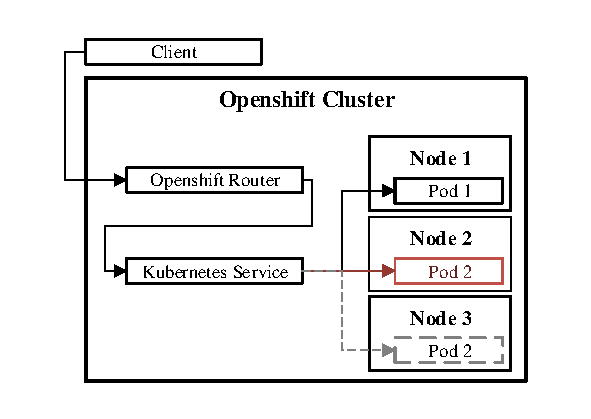
\includegraphics[scale=1]{images/esbd-service-mediation.pdf}
	\caption{Openshift Service mediation}
	\label{fig:esbd-service-mediation}
\end{figure}

Figure \vref{fig:esbd-service-mediation} illustrates a scenario, where the service Pod 2 on Node 2 fails, and gets recreated on Node 3, whereby it gets a new IP address assigned. The Kubernetes Service is aware, that Pod 2 has been recreated on Node 3, and will balance the requests to the recreated Pod 2 located on Node 3, when Pod 2 is fully up and running. A Kubernetes Service performs a simple mediation by abstracting service Pods via service names, and load balancing of the requests to the service Pods depending on the chosen algorithm. \\

With an ESB, there is no central mediator needed, because an ESB is a distributed architectural model, which has no central component like a Hub and Spoke architecture. If message translation is needed, because of a consumer incapability of supporting the ESB used message format and protocols, then an adapter and message translator is needed, as discussed in Section \vref{sec:esbd-adap-trans-service}. \\

The following sections will discuss the tasks introduced in the beginning of this chapter, and will show, that these task can be performed on the implemented prototype.

\section{Managing Multiple Environments}
\label{sec:esbd-multiple-env}
An ESB is commonly hosted on multiple environments, whereby at least one productive and one testing environment should be present. These environments were commonly a VM, which provided the runtime environment for the ESB middleware. As the prototype shows, the environment is now represented by an Openshift Project, which can be reproduced via scripts as discussed in Section \vref{sec:esbi-openshift}. \\

The services hosted on the ESB are using Fuse Integration Service 2.0 and its provided tooling, which ensure, that the services are properly encapsulated in a container, and are properly managed in Openshift. Therefore, the service developers provide the necessary Openshift Templates, which has the effect, that the operators have no interaction with the service artifacts and service runtime environments anymore. Operators have to manage
\begin{itemize}
	\item the Openshift Project, which contains the services,
	\item the Openshift ConfigMaps, which hold the service non-sensitive configuration,
	\item and the Openshift Secrets, which hold the sensitive service configuration.
\end{itemize} 
\ \\
Figure \vref{fig:esbd-multi-stage-env} illustrates the management and provisioning of multiple environments for an ESB, whereby the environment is represented by an Openshift Project. The Management Server pulls the scripts and Openshift Templates from a VCS Server, and the configurations from a Configuration Server, and uses them to provision new Openshift Projects, or manage existing ones. The scripts and Openshift Templates are separated from the configurations, which are providing the values for the scripts and Openshift Template-Parameters. With such an approach, the infrastructure becomes reproducible, versioned, and therefore consistent and disposable. These characteristics of IaC have been discussed in Chapter \vref{cha:iac}.
\newpage 

\begin{figure}
	\centering
	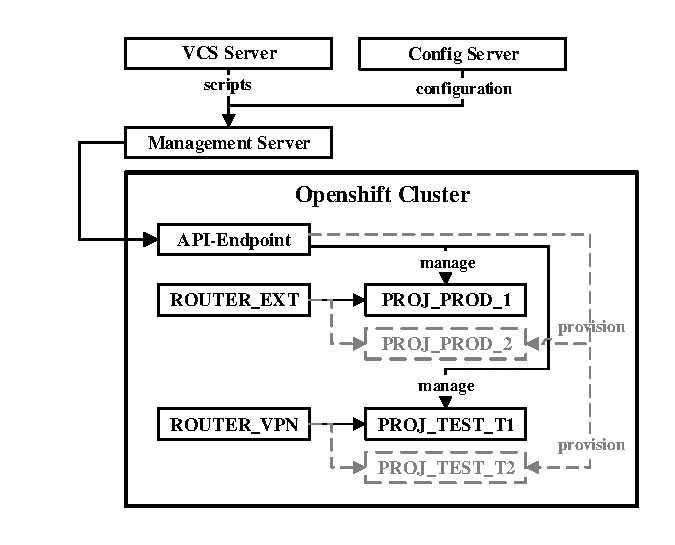
\includegraphics[scale=1]{images/esbd-multi-stage-env.pdf}
	\caption{Management and provisioning of multiple environments}
	\label{fig:esbd-multi-stage-env}
\end{figure}

The interaction of the Management Server, VCS Server and Configuration Server, as illustrated in Figure \vref{fig:esbd-multi-stage-env}, is similar to the Figure \vref{fig:reproduce-infrastructure}, which illustrated how a system can be reproduced with parametrized templates and an IaC tool. The Openshift CLI provides functionality to manage Openshift Objects, which is what needs to be done, when providing an environment in form of an Openshift Project.  \\

Table \vref{tab:esbd-multi-stage-env} compares the Openshift and JBoss EAP contained mechanisms, which provide the listed infrastructure features. As illustrated in the table, Openshift provides networking and isolation features, which are provided to JBoss EAP by its hosting environment such as a VM. Except of the networking and isolation feature, JBoss EAP supports all other features either natively or by supporting a third party library. Nevertheless, Openshift combines all features in one platform, and makes them manageable via Openshift Templates and the Openshift CLI. \\

Openshift runs Docker Containers, and therefore the programming language, the service was implemented with, doesn't matter, as long as the services can run in a container. Also, services hosted on PaaS platforms communicate via standard Protocols such as HTTP, which is commonly supported by almost any programming language. JBoss EAP on the contrary, runs only Java applications.
\newpage

{\renewcommand{\arraystretch}{1.2}%
\begin{table}[h]
	\begin{tabularx}{\textwidth}{ X|X|X }	
	  \textbf{Feature}                  & \textbf{Openshift}         & \textbf{JBoss EAP} \\  \hline
	  \textit{Staging}                  & Openshift Project          & Server Instance \\  \hline
	  \textit{Management}               & Openshift CLI              & JBoss CLI \\
	                                    & Openshift Web-Console      & JBoss Web-Console \\
	                                    & Openshift REST-API         & \\  \hline
	  \textit{Networking}               & Openshift Project          & None (external) \\
	                                    & Openshift Service          & \\  
	                                    & Openshift Route            & \\  
	                                    & Openshift Router           & \\  \hline
	  \textit{Isolation}                & Openshift Project          & None (external) \\  \hline
	  \textit{Configuration/Secrets}    & Openshift ConfigMaps       & Java System-Properties  \\
	                                    & Openshift Secrets          & Environment Variables \\
	                                                                && Password Vault \\  \hline
	  \textit{Service Distribution}     & Openshift Worker-Node      & Single JVM \\ 
			                                                        && Karaf \\  
			                                                        && OSGI \\  \hline
	  \textit{Service Roll-out}         & Recreate                   & Framework dependent, \\ 
			                            & Rolling                    & normally recreate \\ \hline
	  \textit{Language Support}         & All runnable in containers & Java \\
	\end{tabularx}
	\caption{Infrastructure feature comparison}
	\label{tab:esbd-multi-stage-env}
\end{table}}

The next section will discuss the service security within an Openshift Project, which can be managed the same way, as discussed in this section. Additionally to the security, provided by the isolation feature of an Openshift Project, the Management Server of Figure \vref{fig:esbd-multi-stage-env} could also manage custom security configurations, which can be managed via the Openshift CLI as well. 

\section{Managing Service Security}
\label{sec:esbd-service-security}
With a common ESB middleware, the services are protected by running within a single runtime environment, or by security features provided by a supported third party library. In an Openshift Project, the services are implicitly protected by being isolated in a Kubernetes Namespace, as discussed in Section \vref{sec:paas-openshift-project}, whereby the namespace of an Openshift Project cannot be accessed by other Openshift Projects without additional configuration. Services, which are supposed to be accessible from external networks, have to be explicitly exposed via an Openshift Route, which can handle secured connections, similar to an reverse proxy.
\newpage

\begin{figure}[htbp]
	\centering
	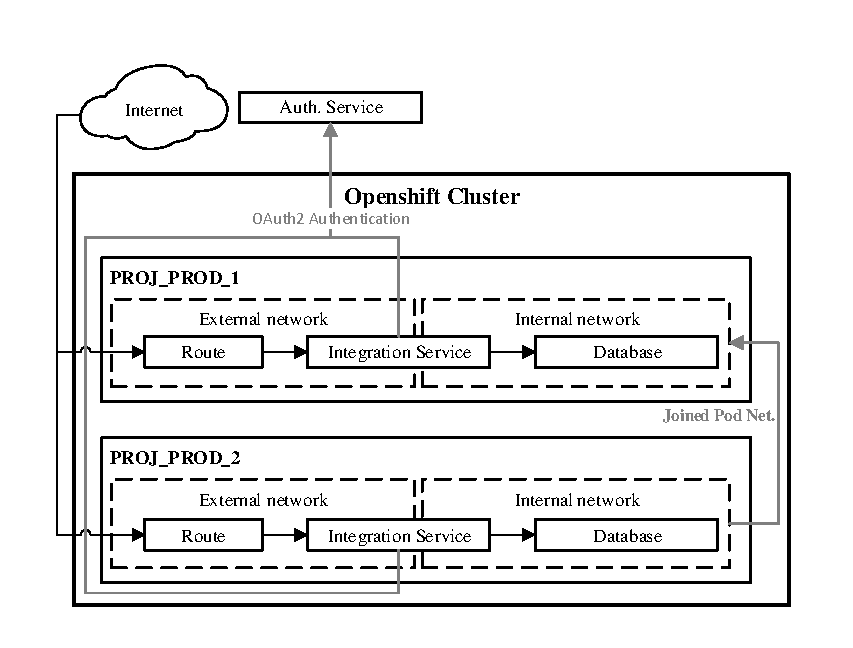
\includegraphics[scale=1]{images/esbd-service-security.pdf}
	\caption{Service security in an Openshift Project}
	\label{fig:esbd-service-security}
\end{figure}
\ \\
Figure \vref{fig:esbd-service-security} illustrates an example, similar to the implemented prototype, whereby two Openshift Projects host the same services, and where the Pod Networks of the two Openshift Projects are joined. The joined Pod Networks allow services hosted in project PROJ\_PROD\_2 to access services hosted in project PROJ\_PROD\_1 by their fully qualified service name. The fully qualified service name has the form of \mentionedtext{<service>.<project\_namespace>.svc.cluster.local}. Joining two Pod Networks is performed by Openshift Cluster administrators, and cannot be performed by developers. \\

Additionally to the isolation of the services within the Openshift Project, the Integration Service is secured via OAuth2, whereby the resource access is controlled by a central Authentication Server. On the one hand, the services are isolated within a Kubernetes Namespace, and on the other hand, additional security, such as access control, has to be provided by the service itself, because Openshift doesn't provide such a feature. It is not meant to isolate services from each other within an Openshift Project, because an Openshift Project, in particular a Kubernetes Namespace, should only contain a set of services, which don't have to be isolated from each other. \\
\newpage

Table \vref{tab:esbd-service-security} compares the Openshift and JBoss EAP contained mechanisms, which provide the listed security features. As illustrated in the table, Openshift doesn't provide any support for access control on the service level, which is normal for a PaaS platform, such as Openshift. The services, running in Docker Containers on an Openshift Cluster, have to implement access control, or have to use third party frameworks, such as the Keycloak Adapter, which provides access control features as discussed in Section \vref{sec:esbi-security}. JBoss EAP on the other hand is a Java Application-Platform, which provides support for access or user control for several providers. 

{\renewcommand{\arraystretch}{1.2}%
	\begin{table}[h]
		\begin{tabularx}{\textwidth}{ X|X|X }	
			\textbf{Feature}                 & \textbf{Openshift}      & \textbf{JBoss EAP} \\  \hline
			\textit{Network Isolation}       & Openshift Project       & None (VM) \\  \hline
			\textit{HTTPS}                   & Openshift Router        & Reverse Proxy \\
			                                 & Openshift Route         & Endpoint Configuration \\  \hline
            \textit{Access Control}          & None (external)         & Endpoint Configuration \\
                                                                      && Internal User-Database \\ 
                                                                      && External User-Database \\  \hline
            \textit{Single-Sign-On}          & None (external)         & Endpoint Configuration \\
                                                                      && Several SSO providers \\  \hline
		\end{tabularx}
		\caption{Security feature comparison}
		\label{tab:esbd-service-security}
\end{table}}

Openshift doesn't provide access control features to secure service resources, but provides security features such as user/group/role management, project permission management, Pod Network management, or quota management for Openshift Objects, such as Replication Controllers. Openshift uses Software Defined Networks (SDNs), whereby 
the services don't have to handle communication security, because the Openshift Cluster will take care of it. Exposed services are connected to an Openshift Route, whereby the Openshift Route, which acts as the reverse proxy, applies security to the communication on the external network. Within the isolated Pod Network, the services don't have to handle communication security, because this is handled by the Openshift Cluster. 

\section{Managing Multiple Service Versions}
\label{sec:esbd-multi-version-service}
Sometimes it is necessary to run multiple versions of a service, for instance, if a new version is released, or if a consumer is not capable of migrating to the new version, but provides a significant business value for the enterprise. Openshift provides mechanisms to run multiple versions of a service in several ways. Figure \vref{fig:esbd-service-multiple-versions} illustrates some scenarios for running multiple service versions on Openshift, whereby the illustrated scenarios of PROJ\_1 and PROJ\_2 are possible, because the old service version is N-1 compatible. N-1 compatibility means, that the service in the old version is capable of reading data written by the service in the new versions.
\newpage

\begin{figure}[htbp]
	\centering
	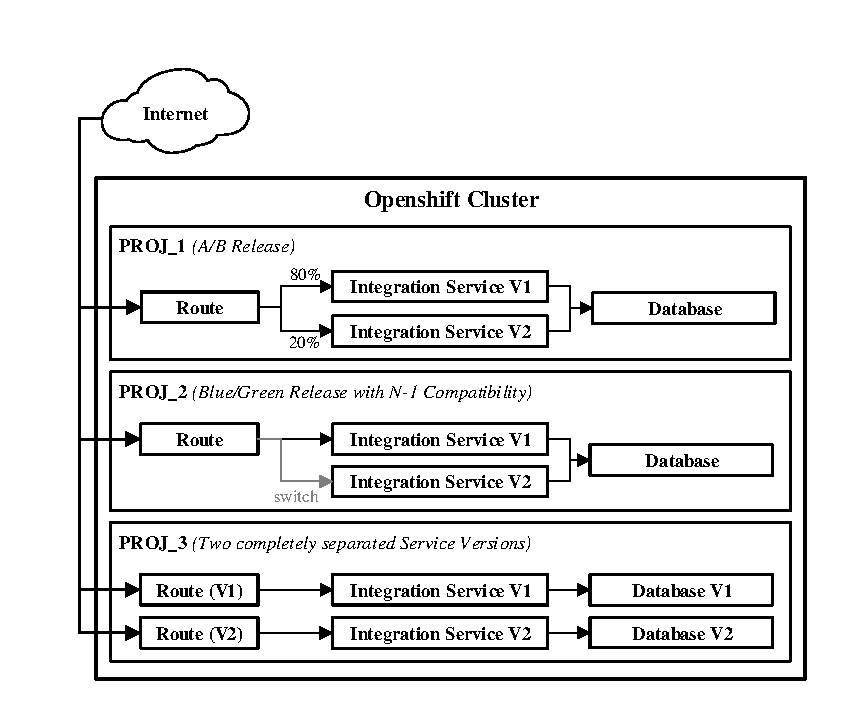
\includegraphics[scale=1]{images/esbd-service-multiple-versions.pdf}
	\caption{Running multiple service versions on Openshift}
	\label{fig:esbd-service-multiple-versions}
\end{figure}

\emph{PROJ\_1} of Figure \vref{fig:esbd-service-multiple-versions} illustrates an A/B Release, which is used to run the old and new version of a service in parallel, whereby a portion of the service consumers get access to the new version, while the rest of the service consumers are still using the old version. A/B Releases are used to validate the new version in the production environment, before fully releasing it to all consumers. In this scenario, the requests are load balanced by the Openshift Route to either the new or old service version. \\ 

\emph{PROJ\_2} of Figure \vref{fig:esbd-service-multiple-versions} illustrates a Blue/Green Release, which is used to run the old and the new version of a service in parallel, whereby the Openshift Route switches between the old and new service version. In this scenario, all service consumer access the same service version, which is currently accessible by the Openshift Route. \\

\emph{PROJ\_3} of Figure \vref{fig:esbd-service-multiple-versions} illustrates two service versions running completely separated in parallel, whereby both versions are accessible via their own Openshift Route. This scenario is not a release scenario, and should be used if multiple service versions have to be provided, for instance, if a customer cannot switch to the new version, but provides a significant business value to the enterprise. \\

Table \vref{tab:esbd-service-multiple-versions} compares the Openshift and JBoss EAP contained mechanisms, which provide the listed release features. Multiple service versions on an Openshift Cluster are represented by separate Openshift Service objects, whereby with JBoss EAP, multiple service versions are either represented by separate JBoss EAP instances, or deployment contexts on a single JBoss EAP instance. With JBoss EAP version switching and weighted routing can be performed by an external reverse proxy, which in Openshift can be performed by an Openshift Route.

{\renewcommand{\arraystretch}{1.2}%
 \newcolumntype{m}{>{\hsize=.32\hsize}X}%
	\begin{table}[h]
		\begin{tabularx}{\textwidth}{ X|X|X }	
			\textbf{Feature}                  & \textbf{Openshift}      & \textbf{JBoss EAP} \\  \hline
			\textit{Multiple Service Versions}& Openshift Service       & Multiple EAP instances \\
											  & Openshift Route    	    & Multiple deployment contexts \\ \hline
			\textit{Weighted Routing}         & Openshift Route         & None (external) \\  \hline
			\textit{Version Switch}           & Openshift Route         & None (external) \\  \hline
		\end{tabularx}
		\caption{Release feature comparison}
		\label{tab:esbd-service-multiple-versions}
\end{table}}

JBoss EAP is an application platform for Java applications, which provides a runtime environment for Java applications, but no networking features, as shown in Table \vref{tab:esbd-multi-stage-env}, and therefore no routing feature. JBoss EAP can be configured to act as a reverse proxy, but cannot act as the reverse proxy for applications hosted on the same JBoss EAP instance. As Figure \vref{fig:esbd-service-multiple-versions} illustrates, the implemented prototype can run multiple versions of the hosted services, and supports the implementation of release models such as A/B or Blue/Green Releases.

\section{Managing Migration of Public API}
\label{sec:esbd-multi-stage-env}
This section will discuss the management of services public API, which is crucial, when it comes to distributed services. Changes made on the public API of a service can break the functionality of an application, the service is part of, or break the functionality of an external application, which depends on this service. The public API is the API the service exposes, which could only be consumed by internal consumers, but has to be managed the same way, as the API would be exposed to external consumers. There are several ways to migrate a public API, whereby some of them will be discussed in the further sections. \\  

Services running on an Openshift Cluster are completely separated from each other and have their own life-cycle. Therefore, they have to provide a public API, which can be consumed by other services. The public API has to be designed properly in the first place, as well as the management of its migrations. At least, the last both versions will have to be supported, to give the developers of the consuming services enough time to apply to the migrations performed on the public API. Commonly, a service has two versions, the service release version, and the service API version, which is allowed to remain the same over multiple service releases. 
\newpage

The following sections will discuss the different ways to migrate the public API of a service.

\mysubsubsection{URL Query-Parameter Versioning}
Multiple versions of a public API can be managed via a URL Query-Parameter, whereby the URL Query-Parameter defines the version to use of a single API Operation. The URL \inlineBash{http://localhost/api/users?version=2} illustrates how to access a specific version of an API Operation via a URL Query-Parameter. Table \vref{tab:esbd-service-api-query-param} shows the Pros and Cons of API Versioning with URL Query-Parameters.

{\renewcommand{\arraystretch}{1.2}%
	\begin{table}[h]
		\begin{tabularx}{\textwidth}{ X|X }	
			\textbf{Pros}                 & \textbf{Cons}    \\  \hline
			Single resource address       & Data and control parameters are mixed  \\ \hline
			Supported by all browsers     & Version as data parameter not possible \\ \hline
			Easy to understand            & No declarative mapping with JAX-RS     \\ \hline
			Easy to implement             & Manual switch between API Operations   \\ \hline
		\end{tabularx}
		\caption{Pros and Cons of URL Query-Parameter Versioning}
		\label{tab:esbd-service-api-query-param}
\end{table}}

\mysubsubsection{HTTP Header Versioning}
Multiple version of a public API can be managed via HTTP Headers in the following listed ways:
\begin{itemize}
	\item New HTTP Header \\
	e.g. \inlineBash{Version: 2}
	\item Additional field in the Accept-Header \\
	e.g. \inlineBash{Accept: application/json; version=2}
	\item Enhanced Media-Type \\
	e.g. \inlineBash{Accept: application/vnd.app.model.v1+json;qs=0.9}
\end{itemize}
\ \\
The approach of HTTP Header Versioning brings in more flexibility, but also makes the API Versioning harder to understand for consumers, especially when quality of service is used in the HTTP Accept-Headers of multiple API Operations. Table \vref{tab:esbd-service-api-http-header} shows the Pros and Cons of API Versioning with HTTP Headers.

{\renewcommand{\arraystretch}{1.2}%
\begin{table}[h]
	\begin{tabularx}{\textwidth}{ X|X }	
		\textbf{Pros}                         & \textbf{Cons}                  \\ \hline
		Single resource address               & Header handling needed         \\ \hline  
		No mix of data and control parameters & Harder to understand           \\ \hline
		Declarative mapping with JAX-RS       & No enhanced Media-Type in HTML \\ \hline
		Easy to implement                     & More difficult to test         \\ \hline
	\end{tabularx}
	\caption{Pros and Cons of HTTP Header Versioning}
	\label{tab:esbd-service-api-http-header}
\end{table}}

\mysubsubsection{Path Versioning}
The easiest way to manage multiple versions of a public API is Path Versioning, whereby the whole API is versioned, instead of single API Operations. The URL \inlineBash{http://localhost/api/v2/users} illustrates how to access a specific version of an API Operation via a Path version. The Path Versioning is the most used approach to version a public API, because of its simplicity to realize.  Table \vref{tab:esbd-service-api-path} shows the Pros and Cons of API Versioning with Path versions.

{\renewcommand{\arraystretch}{1.2}%
	\begin{table}[h]
		\begin{tabularx}{\textwidth}{ X|X }	
			\textbf{Pros}                         & \textbf{Cons}                         \\ \hline
			Easy to implement                     & Multiple resource addresses           \\ \hline
			Easy to understand                    & Declarative mapping with JAX-RS       \\ \hline
			No mix of data and control parameters & Version actually not part of resource \\ \hline
			Easy to switch between versions       & Latest version unknown                \\ \hline
		\end{tabularx}
		\caption{Pros and Cons of Path Versioning}
		\label{tab:esbd-service-api-path}
\end{table}}

The prototype uses Swagger for documenting the services public API, as discussed in Section \vref{sec:esbi-api}, whereby Swagger is used to generate the Swagger Documentation and clients. One advantage of a Swagger generated client is, that developers work with generated classes and interfaces, and therefore, developers work with a typed client, which will cause compile errors on breaking API changes. The API changes can be performed in a way, whereby developers will not have to change anything in their source code, but could also be performed in a way to cause compile errors, which force the developers to apply to the breaking API changes. If the client is implemented by hand and not generated by a tool, then developers will have to ensure that the implemented client is in sync with the currently used API version.

\section{Managing Adapters and Message Translator as Services}
\label{sec:esbd-adap-trans-service}
Adapters and Transformers are part of the EI Patterns, whereby the Adapter is used to couple an application to a message bus, and the Transformer is used to transform messages from the application supported format to the message bus supported format and vice versa. The Adapter and Message Translator can either be  located at the external service, or can be located in the messaging system, the external service connects to. Commonly, a message bus system is implemented to use one form of communication, such as REST, and one form of data representation. If external services need to access the message bus, but don't support the message bus protocol and data format, then Adapters and Message Translators are needed, to connect the external service to the message bus. \\

Figure \vref{fig:esbd-service-adapter} illustrates how the prototype could be integrated with external applications via an Adapter and Message Translator. If the Adapter and Message Translator are located at the external service, then the Adapter and Message Translator have to be provided in the programming languages, the external services are implemented with. If the Adapter and Message Translator are located in the Openshift Project, then they can be implemented in the programming language of choice.

\begin{figure}[htbp]
	\centering
	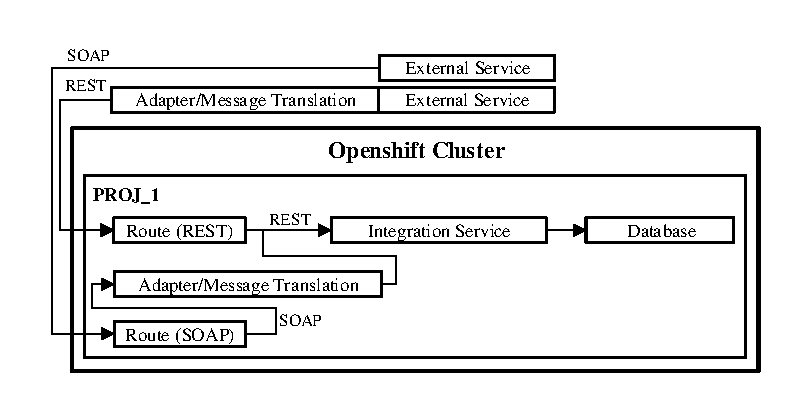
\includegraphics[scale=1]{images/esbd-service-adapter.pdf}
	\caption{External services integrated via an adapter}
	\label{fig:esbd-service-adapter}
\end{figure}

The Adapter and Message Translator have to be implemented as a standalone application (microservice), which for instance can be realized in Java with the Camel framework, which provides an API for implementing EI Patterns, and is capable of running as a standalone application. The adapter and message translator application can be hosted as a separate Openshift Service, or can be added to the service Pod as a so called side-by container, which proxies the requests to the actual container.  \\

\section{Further Work}
\label{sec:esbd-furhter-work}
During writing this thesis and the implementation of the prototype, Red Hat has released its new version of the JBoss Fuse platform, which now is based on Openshift, and is called Red Hat Fuse 7. Red Hat Fuse 7 enhances Openshift with features for implementing an ESB, whereby the main goal is to provide non-technical personal the possibility to create integrations. Red Hat Fuse 7 provides IPaaS features, by providing a low/no code UI, which allows to create integrations without the need to write a single line of code. \\

The next step is to implement an ESB with Red Hat Fuse 7, to see the differences between the manual approach, represented by the prototype, and the approach using IPaaS provided features. Red Hat Fuse 7 should make it easier for enterprises to create integrations to external services, as well as the management of these integrations.   

%%%----------------------------------------------------------
\appendix                                         % appendix 
%%%----------------------------------------------------------

%\chapter{Technical Details}
\label{app:TechnicalDetails}



	% technical supplements
%\chapter{CD-ROM/DVD Contents}
\label{app:cdrom}


	% contents of the CD-ROM/DVD
%\chapter{Questionnaire}
\label{app:Questionnaire}





	% chronological list of changes
%\chapter{\latex Source Code}
\label{app:SourceCode}

	% source text of this document

%%%----------------------------------------------------------
\MakeBibliography                     				% references
%%%----------------------------------------------------------
%%% special page for checking print size --------------------
%\chapter*{Check Final Print Size}

\begin{center}
{\Large --- Check final print size! ---}

\bigskip

\calibrationbox{100}{50} % width/height of box in mm

\bigskip

{\Large --- Remove this page after printing! ---}

\end{center}



%%%----------------------------------------------------------
\end{document}
%%%----------------------------------------------------------